\documentclass[a4paper,fleqn]{book}

\usepackage{graphicx,amsfonts,psfrag,fancyhdr,layout,appendix,subfigure,amsmath}
\usepackage[sectionbib]{natbib}
\usepackage{chapterbib}

% Set equal margins on book style
\setlength{\oddsidemargin}{53pt}
\setlength{\evensidemargin}{53pt}
\setlength{\marginparwidth}{57pt}
\setlength{\footskip}{30pt}

% Redefine plain page style
\fancypagestyle{plain}{
\fancyhf{}
\renewcommand{\headrulewidth}{0pt}
\fancyfoot[LE,RO]{\thepage}
}

% Code for creating empty pages
% No headers on empty pages before new chapter
\makeatletter
\def\cleardoublepage{\clearpage\if@twoside \ifodd\c@page\else
    \hbox{}
    \thispagestyle{plain}
    \newpage
    \if@twocolumn\hbox{}\newpage\fi\fi\fi}
\makeatother \clearpage{\pagestyle{plain}\cleardoublepage}


% Define pagestyle
\pagestyle{fancy}
\fancyhf{}
\renewcommand{\chaptermark}[1]{\markboth{ \emph{#1}}{}}
\fancyhead[LO]{}
\fancyhead[RE]{\leftmark}
\fancyfoot[LE,RO]{\thepage}

% Dutch style of paragraph formatting, i.e. no indents. 
\setlength{\parskip}{1.3ex plus 0.2ex minus 0.2ex}
\setlength{\parindent}{0pt}

% Less detailed TOC
\setcounter{tocdepth}{2}

\makeindex

% Document starts here
\begin{document}

\frontmatter

\title{A Short Course in Fixed Income Pricing, Portfolio Management, and Trading}
\author{Joseph Clark}

\maketitle
\date{}

%\include preface

% Remove parskip for toc
\setlength{\parskip}{0ex plus 0.5ex minus 0.2ex}
\tableofcontents

% Dutch style of paragraph formatting, i.e. no indents.
\setlength{\parskip}{1.3ex plus 0.2ex minus 0.2ex}

\mainmatter
% Adjustments headers
\fancyhead[LO]{\leftmark}
\fancyhead[RE]{\emph{Chapter \thechapter}}

\chapter{Introduction}

Much of the capitalist economy is funded on credit. Each different borrower, in each different currency, for loans of different lengths of time, borrows on different terms. Fixed  income is the study of how to price and manage these differences. 

This is a short course through theory and practice of fixed income markets in three chapters:


\textbf{Chapter 1: Pricing}: Methods for pricing different loans and combinations of loans.\\
\textbf{Chapter 2: Portfolio Management:} Methods for managing a portfolio of loans.\\
\textbf{Chapter 3: Trading:} Methods for trading loans to achieve desirable objectives.



\chapter{Pricing}

\section{The basics}

People who lend money often insist on being paid a rental rate. The rate depends on the period of the loan, the person, the currency, and a number of other factors. Loans are often resold into secondary markets and traded like any other financial asset. The study of money loans is called \textbf{fixed income} (or \textbf{fixed interest}) because the amount of money repaid is generally fixed by agreement, in comparison to other assets where future financial flows are uncertain.

Fixed income is useful to know:  The pricing and analysis of many other products incorporates information about the rental price of money, so it's difficult to understand what's going on with options or futures or more exotic things without knowing a bit about the debt markets.

Three objects will concern us here: \textbf{bonds}, \textbf{zero rates}, \textbf{forward rates}, and \textbf{swap rates}. Understanding these and how to convert between them is fundamental to understanding fixed income markets. We'll start by assuming that all loans are the same except for when they are taken out and repaid.

\subsection{Notation}
Start with some notation. Let $y(t)$ be the interest rate for a loan made now and repaid in $t$ years. The curve for all $t$ is called the \textbf{zero curve} and the component rates \textbf{zero rates}. This is short for `zero coupon', but don't worry about that for now.

Now let $f(t_1,t_2)$ be the interest rate for a loan made at time $t_1$ and paid back at time $t_2$. These are called \textbf{forward rates}.

Unless otherwise noted all rates from here will be continuously compounded. The appendix contains a reminder of how continuous compounding works and how to convert between discrete and continuous compounded rates so $N$ dollars borrowed at rate $y$ for $T$ periods will compound to

\[N\exp (yT) \]


\section{Converting between zero rates and forward rates}


\subsection{General case}

If we have two \textit{zero rates} $y(t_1)$ and $y(t_2)$ we can determine the forward rate $f(t_1,t_2)$ -- the interest rate on a loan taken out at $t_1$ and repaid at $t_2$ -- using an arbitrage argument. The essence of this argument is that it should cost the same to borrow from now to $t_1$, and then at the forward rate from $t_1$ to $t_2$, as it does to simply borrow from now to $t_2$. If this were not true there would be an arbitrage.

In more concrete terms it should cost the same to take out a loan for two years as to take out a loan for one year, and another in a years time at the forward rate (see figure \ref{frArb}) . This gives us the formula for forward rates:

\begin{figure}[htbp]
\begin{center}
  \includegraphics[width=5in]{pics/zt1t2_llb.png} \\
  \caption{Forward rate arbitrage: borrow long, lend short}
\label{frArb}
\end{center}
\end{figure}


\begin{center}
(loan for $t_2$ periods)  = (loan for $t_1$ periods)(loan for $t_2-t_1$ periods)
\[\Rightarrow \exp(y(t_2)t_2) = \exp(y(t_1)t_1)\exp(f(t_1,t_2)(t_2-t_1)) \]
We can solve to get any forward rate:
\begin{equation}f(t_1,t_2) = \frac{y(t_2)t_2-y(t_1)t_1}{t_2-t_1}  \label{fRates}\end{equation}
\end{center}


\subsection{Example} Suppose that $y(1) = 0.05$ and $y(2) = 0.075$. We can see immediately that

\[f(1,2) = \frac{0.075*2-0.05*1}{2-1} = 0.1 \]


Which is to say that the one year rate one year from now (from year one to year two) should be 10\%.

\subsection{Forward rate arbitrage}

If the forward and zero rates does not conform to \ref{fRates} there will be arbitrage. We'll work through a couple of examples to see how this works.

But what if it isn't? What if instead $f(1,2)=0.11$? Then we would have the following arbitrage:
\begin{center}
\begin{tabular}{|c|c|}
  \hline
  % after \\: \hline or \cline{col1-col2} \cline{col3-col4} ...
  time & transaction \\
  \hline
  now & Borrow \$1 for 2 years at 0.075 \\
   & Lend \$1 for 1 year at 0.05 \\
   \hline
  1 & Receive \$ 1$\exp(0.05*1)$ \\
   & Lend \$1$\exp(0.05*1)$ \\
  \hline
  2 & Receive \$1$\exp(0.05*1)\exp(0.11*(2-1))$ \\
   & Repay  \$1 $\exp(0.075*2)$ \\
  \hline
  Profit & \$1$\exp(0.05*1)\exp(0.11*(2-1))-\$1 \exp(0.075*2) = \$0.0117$ \\
  \hline
\end{tabular}
\end{center}

\begin{figure}[htbp]
\begin{center}
  \includegraphics[width=3in]{pics/zt1t2_bbl.png} \\
  \caption{Forward rate arbitrage: borrow short, lend long}
\label{frArb2}
\end{center}
\end{figure}



If instead $f(1,2)=0.09$ we would do the opposite to last time:\\
\begin{center}
\begin{tabular}{|c|c|}
  \hline
  % after \\: \hline or \cline{col1-col2} \cline{col3-col4} ...
  time & transaction \\
  \hline
  now & Lend \$1 for 2 years at 0.075 \\
   & Borrow \$1 for 1 year at 0.05 \\
   \hline
  1 & Repay \$1$\exp(0.05*1)$ \\
   & Borrow \$1$\exp(0.05*1)$ @ 0.11 \\
  \hline
  2 & Repay \$1$\exp(0.05*1)\exp(0.11*(2-1))$ \\
   & Receive  \$1 $\exp(0.075*2)$ \\
  \hline
  Profit & \$1 $\exp(0.075*2)$-\$1$\exp(0.05*1)\exp(0.09*(2-1)) = \$0.0116$ \\
  \hline
\end{tabular}
\end{center}

The general version of the two arbitrages for $y(t_1)$,$y(t_2)$, and $f(t_1,t_2)$ for $0<t_1<t_2$\\

If \[f(t_1,t_2) < \frac{y(t_2)t_2-y(t_1)t_1}{t_2-t_1} \]

then\\
\begin{center}
\begin{tabular}{|c|c|}
  \hline
  % after \\: \hline or \cline{col1-col2} \cline{col3-col4} ...
  time & transaction \\
  \hline
  now & Borrow \$1 for $t_2$ years at $y(t_2)$ \\
   & Lend \$1 for $t_1$ years at $y(t_1)$ \\
   \hline
  1 & Receive \$1$\exp(y(t_1)*t_1)$ \\
   & Lend \$1$\exp(y(t_1)*t_1)$ at $f(t_1,t_2)$ \\
  \hline
  2 & Receive \$1$\exp(y(t_1)*t_1)\exp(f(t_1,t_2)*(t_2-t_1))$ \\
   & Repay  \$1 $\exp(y(t_2)*t_2)$ \\
  \hline
  Profit & \$1$\exp(y(t_1)*t_1)\exp(f(t_1,t_2)*(t_2-t_1))-\$1 \exp(y(t_2)*t_2)>0$  \\
  \hline
\end{tabular}
\end{center}

If \[f(t_1,t_2) > \frac{y(t_2)t_2-y(t_1)t_1}{t_2-t_1} \]

then\\
\begin{center}
\begin{tabular}{|c|c|}
  \hline
  % after \\: \hline or \cline{col1-col2} \cline{col3-col4} ...
  time & transaction \\
  \hline
  now & Lend \$1 for $t_2$ years at $y(t_2)$ \\
   & Borrow \$1 for $t_1$ years at $y(t_1)$ \\
   \hline
  1 & Repay \$1$\exp(y(t_1)*t_1)$ \\
   & Borrow \$1$\exp(y(t_1)*t_1)$ at $f(t_1,t_2)$ \\
  2 & Repay \$1$\exp(y(t_1)*t_1)\exp(f(t_1,t_2)*(t_2-t_1))$ \\
   & Receive  \$1 $\exp(y(t_2)*t_2)$ \\
  \hline
  Profit & $\$1 \exp(y(t_2)*t_2)-\$1 \exp(y(t_1)*t_1)\exp(f(t_1,t_2)*(t_2-t_1))>0$  \\
  \hline
\end{tabular}
\end{center}

This should be enough to convince us that the relationship in \ref{fRates} holds nearly exactly. Forward rate arbitrage, when it exists, will be gobbled up very quickly amongst the deep liquidity and tight spreads of the bond markets.

\section{Determining zero rates from bond prices}

Life would be easier if all bonds were simple borrow-at-$t_1$-repay-at-$t_2$ type arrangements. If they were the relationship between the price and yield of of a bond would be

\begin{eqnarray*}
P(0) &=& F\exp (-y(t)t)\\ \mbox{ or, in terms of yield, }\\
y(t) &=& -\ln \left( \frac{P(0)}{F} \right)1/t
\end{eqnarray*}

So a bond that paid \$100 in 5 years time which currently traded at \$67 could be revealed to have a yield of

\[0.0801 = -\ln \left( \frac{67}{100} \right)1/5\]

But life wasn't meant to be easy, and bonds have a nasty habit of paying a regular sequence of payments (called \textbf{coupons}) and then a final payment (called the \textbf{face value}). This complicates things a bit.

\subsection{Determining the price of a bond with coupons}

\subsubsection{Example}
We might have a 5 year bond with a 6\% coupon and \$100 face value that pays a \$6 coupon every year and \$100 after 5 years. What's the yield and price of this bond?

This bond is really easy to price. We just note that any payment $FV$ that occurs in the future in $t$ years is worth \[PV = F\exp(-y(t)t)  \]
where $y(t)$ is the interest rate

The payments [6,6,6,6,6+100] at times [1,2,3,4,5] are therefore worth
\begin{eqnarray*}P = 6\exp(-y(1)*1)+6\exp(-y(2)*2)\\+6\exp(-y(3)*3)+6\exp(-y(4)*4)\\+(6+100)\exp(-y(5)*5)\end{eqnarray*}

\subsubsection{General case}
In general for a stream of coupons $[C_1,...,C_N]$ at times $[t_1,\ldots,t_N]$ with and a face value of $F$ with rates of

\begin{equation}P = \left[\sum_{j=1}^N C_j\exp(-y(t_j)t_j)\right] + F \exp(-y(t_N)t_N)  \label{bondPrice}\end{equation}

This is the bond pricing formula.

\subsection{Determining the yield of a bond with coupons}

\subsubsection{General case}
The \textit{yield} of a bond is the unique interest rate that satisfies the price. Just drop the argument from the interest rates and solve!

\begin{eqnarray*}
P = \left[\sum_{j=1}^N C_j\exp(-yt_j)\right] + F \exp(-yt_N) \\
y = \ldots
\end{eqnarray*}
It's a bit tricky to solve directly but you get the idea. In practice these problems are solved by choosing a value of $y$ that makes $P- \left[\sum_{j=1}^N C_j\exp(-yt_j)\right] - F \exp(-yt_N)$ as close as possible to zero. This can easily done easily with a spreadsheet or mathematical package.

\subsection{Generating the zero curve from coupon bond prices}

Now the useful part: We will typically have prices for a number of coupon bonds, from which the coupon yields can be fairly easily calculated. It is a bit more difficult to extract the zero rates $y(t)$ from these prices. To do this we use an iterative process called \textbf{bootstrapping}.

Start by noting that all the repayments from a bond, coupons and face value, can be considered in isolation as zero coupon bonds. If we are able to determine the shortest (to maturity) zero rate, we can use it to obtain the next shortest rate, and so on.

\subsubsection{Example} Suppose we have three bonds: a 1/2 year, a 1 year, and a 1.5 year. Each bond pays semi-annual coupons and the face value at maturity. We know the price of each bond, as well as the coupons and face values, and we want to find the zero-coupon rates. The prices are in the table below

\begin{tabular}{|c|c|c|c|c|}
  \hline
  % after \\: \hline or \cline{col1-col2} \cline{col3-col4} ...
  maturity & coupon rate & coupon frequency & face value ($F$) & price ($P$) \\
  \hline
  $t_1 = 0.5$ & 10\%  & semi-annual & 100 & 99 \\
  $t_2 = 1$ & 10\%  & semi-annual & 100 & 96 \\
  $t_3 = 1.5$ & 10\% & semi-annual & 100 & 95 \\
  \hline
\end{tabular}

We can quickly discover the first zero rate $y(0)$ by using the bond pricing formula \ref{bondPrice}. We have

\begin{eqnarray*}
P = \left[\sum_{j=1}^N C_j\exp(-y(t_j)t_j)\right] + F \exp(-y(t_N)t_N) \\
\Rightarrow P(0.5) = \left[C_1\exp(-y(0.5)0.5)\right] + F \exp(-y(0.5)0.5) \\
\Rightarrow y(0.5) &=& \frac{1}{t_1}\ln\left(\frac{F+C}{P(0.5)}\right) \\
&=& \frac{1}{0.5}\ln\left(\frac{100+5}{99}\right) = 0.1177 \\
\end{eqnarray*}

So the zero coupon rate for maturity of 1/2 a year is 11.77\% Splendid.

 Now we can use this to obtain the 1 year zero coupon rate. We again start with the bond pricing formula and substitute in for the one year bond, using our result for $y(0.5)$ from the last step.

\begin{eqnarray*}
P = \left[\sum_{j=1}^N C_j\exp(-y(t_j)t_j)\right] + F \exp(-y(t_N)t_N)\\
\Rightarrow P(1) = \frac{C_1}{\exp(y(0.5)*0.5)} +\frac{F+C_2}{\exp(y(1)*1)}\\
\Rightarrow y(1) &=& \ln \left(\frac{F+C_2}{P(1)-\frac{C_1}{\exp(y(0.5)*0.5)}} \right)\\
 &=& \ln \left(\frac{100+5}{96-\frac{5}{\exp(0.1177*0.5)}} \right) = 0.14
\end{eqnarray*}

Things are going well. Now we have the 1/2 year rate and the 1 year zero rate. Note that this is different from the yields on those two bonds. The zero rates are more informative, which is why we are willing to spend all this trouble obtaining them.

The third step is the same again:

\begin{eqnarray*}
P = \left[\sum_{j=1}^N C_j\exp(-y(t_j)t_j)\right] + F \exp(-y(t_N)t_N)\\
P(1.5) = \frac{C_1}{\exp(y(0.5)*0.5)} +\frac{C_2}{\exp(y(1)*1)}+\frac{F+C_3}{\exp(y(1)*1)}\\
\Rightarrow y(1.5) = 0.1335
\end{eqnarray*}

Now we have all the zero rates. This schedule of rates $y(0.5) = 0.1177$, $y(1)=0.14$, $y(1.5) = 0.1335$ is called the \textbf{zero coupon curve} and represents the continuously compounded interest rates for a simple loans with these maturities.

\subsubsection{General case}
In general for a stream of coupons $[C_1,...,C_N]$ at times $[t_1,\ldots,t_N]$ with and a face value of $F$ the $N$'th zero coupon yield is given by

\begin{equation}
y(t_N) = \frac{1}{t_N} \ln \left( \frac{C_N +F}{P(t_N)-\sum_{i=1}^{N-1}\exp(-C_{j}y(t_j)t_j))} \right)
\end{equation}

\subsubsection{Arbitrage}

If zero rates differ from our calculated zero curve we can construct an arbitrage. To keep things simple lets assume that the bonds in the table are offered and there are also a yield curve $y(0.5)=y(1)=y(1.5)=0.1$. Say we want to arbitrage the 1.5 year bond, we construct the arbitrage by buying the bond financed by a 1.5 year loan at 10\%. We'll get paid three coupons of \$5 each. The first two we'll reinvest at the forward rates $f(0.5,1.5)$ and $f(1,1.5)$. The last one will be paid at maturity along with the face value of \$100.

The forward rates are 

\begin{eqnarray*}
f(t_1,t_2) &=& \frac{y(t_2)t_2-y(t_1)t_1}{t_2-t_1}\\
\Rightarrow f(0.5,1.5) &=& \frac{y(1.5)1.5-y(0.5)0.5}{1.5-0.5}\\
&=& \frac{0.1*1.5-0.1*0.5}{1.5-0.5}\\
&=& 0.1\\
            f(1,1.5) &=& \frac{y(1.5)1.5-y(1)1}{1.5-1}\\
            &=& \frac{0.1*1.5-0.1*1}{1.5-1}\\
            &=& 0.1
\end{eqnarray*}


The arbitrage looks like this

\begin{center}
\begin{tabular}{|c|c|}
  \hline
  % after \\: \hline or \cline{col1-col2} \cline{col3-col4} ...
  time & transaction \\
  \hline
  now & Borrow \$95 for 1.5 years at 0.1 \\
   & Buy 1.5 year bond \\
   \hline
  0.5 & Receive \$5 coupon \\
   & Invest \$5 coupon at f(0.5,1.5)\\
  \hline
  1 & Receive \$5 coupon \\
   & Invest \$5 coupon at f(1,1.5)\\
  \hline
  1.5 & Receive \$5 coupon \\
      & Receive first reinvested coupon: $5\exp (0.1*1)=5.5259$\\
      & Receive first reinvested coupon: $5\exp (0.1*0.5)=5.2564$\\
      & Receive \$100 face value\\
      & Repay loan: $95\exp (0.1*1.5) = 110.37$\\
  \hline
  Profit & 5.5259+5.2564+100-110.37 = 0.4122 \\
  \hline
\end{tabular}
\end{center}

\textbf{Exercise:} Construct an arbitrage if the yield curve were $y(0.5)=y(1)=y(1.5)=0.15$

\section{Converting forward rates to swap rates}

A swap is a financial contract to swap a series of payments over time. There are three types of swaps
\begin{enumerate}
\item \textit{Fixed-Fixed}: One fixed payment against another. e.g. pay 1 apple per week for 10 weeks, receive 1 banana per week for 10 weeks.
\item \textit{Fixed-Floating:} One side is fixed and the other side is determined by something that hasn't happened yet. e.g. pay 6\% times \$100 per year for 10 years against the Fed funds rate times \$100 per year for 10 years.
\item \textit{Floating-Floating:} Both sides are floating. e.g. pay RBA cash rate times \$100 per year for 10 years, receive 2\%+ Fed funds rate per year for 10 years.
\end{enumerate}

In the simplest type of swap the floating side of the swap is paid \textit{after} the rate is set. So, for instance, if the agreement is to pay 90 day BBSW, the exchange occurs 90 days after the as yet unknown BBSW is observed. The payment date is sometimes called the \textbf{anniversary date}. 

There are other types of swaps where payments are exchanged on the date that the floating rate is observed. These are called \textbf{in arrears swaps} but they're a bit tricky to price so we won't cover them here.

We'll need a slight change in notation to talk about future spot rates. We'll call $y(t,T)$ the zero rate observed at time $t$ for a loan starting at $t$ and maturing at $T$. In the previous sections we have been talking about rates observed now so $y(1) \equiv y(0,1)$ etc.

An additional irritation is that we will be using both simple (period by period) and continuously compounded rates for reasons that become clear when you look at the hedging arguments. We'll use the subscript $s$ to denote the simple rate. If you lend \$1 at the simple rate $y_s(0,T)$ for $T$ periods you get $\$1(1+y_s(0,T))^T$ back when the loan is due. Simple rates have a straightforward relationship to continuously compounded rates:

\[ y_s(t,T) = e^{y(t,T)}-1\]

\subsection{The big idea}

A swap is a series of known and unknown payments. To price a swap correctly we find instruments to hedge out all the unknown payments. We generally do this with forwards. Once we remove the uncertain elements we can quickly determine the swap rate that gives a present value of zero. Any deviation from this gives us an arbitrage.

Say we agree now at time $t=0$ to borrow \$1 at the forward rate $f(1,2)$ in one year's time. At $t=1$ we can borrow at the agreed rate and lend at the prevailing rate $y(1,2)$. At $t=2$ we repay the forward-price loan for $\$1e^{f(1,2)}$ and receive payment on the other loan for $\$1e^{y(1,2)}$. The payoff is

\[ \$1e^{f(1,2)} -\$1e^{y(1,2)} \]

This trade has a negative exposure to $y(1,2)$. We can use trades like this to offset unwanted exposures to the rate. We can do the trade in reverse to generate the positive exposure. This is the trick we will use to value the floating parts of swaps. 

\subsection{Swap-forward arbitrage}

We'll explore the arbitrage argument with generic one and two period swaps.\\

\textbf{Example: a one period swap}\\

The best place to start is with only one exchange of payments. In this example we agree at $t=0$ to exchange $\$1*y_s(1,2)$ for some swap rate $\$1*SW$ at $t=2$. Note that we pay the $y_s(1,2)$ on the anniversary ($t=2$) one year after we observe it. What should $SW$ be? 

\begin{figure}[htbp]
\begin{center}
  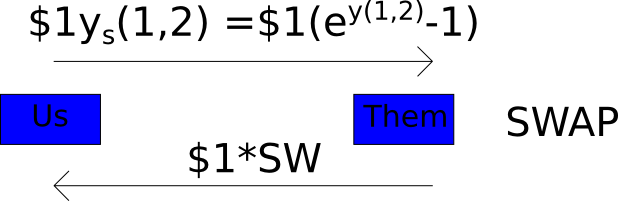
\includegraphics[width=3in]{pics/swap1P.png} \\
  \caption{Swap at t=2}
\label{swap1P}
\end{center}
\end{figure}

The answer comes from an arbitrage argument. We will hedge the floating payment with forwards and then find the swap rate that makes the combined value of all fixed and floating payments equal to zero. If they are not zero we have an arbitrage.

Say we recieve the fixed rate and pay the floating rate. The most obvious (and correct) hedge is a forward contract to borrow \$1 from $t=1$ to $t=2$. This rate is $f(1,2)$. At $t=1$ we lend out this \$1 for a year at the prevailing rate $y(1,2)$.

The table below gives the story of the swap and the hedge:

\begin{tiny}
\begin{tabular}{|c|c|c|}
\hline
time & contract/action & cashflow\\
\hline
0 & \begin{tabular}{c}Enter swap to pay $\$1*y_s(1,2)$ and receive $\$1*SW$\\ Enter forward to borrow \$1 at $f(1,2)$\\ \end{tabular} & 0\\
\hline
1 & \begin{tabular}{c}Borrow \$1 at $f(1,2)$\\ Lend \$1 at $y(1,2)$ \end{tabular} & 0\\
\hline
2 & & \begin{tabular}{c}Pay $\$1e^{f(1,2)}$ from loan\\ Receive $\$1e^{(y(1,2)}$ from loan\\ Pay $\$1y_s(1,2)$ from swap \\ Receive $\$1SW$ from swap\\  \end{tabular}\\
\hline
\end{tabular}
\end{tiny}

We can divide the cashflows into those coming from loans (including the loan at the forward rate) and the fixed and floating side of the swap. We'll also discount everything at $t=2$ by $y(0,2)$:

\begin{tiny}
\begin{tabular}{|c|c|c|c|}
\hline
time & value of loans & value of floating & value of fixed\\
\hline
0 & 0 & 0 & 0\\ 
1 & 0 & 0 & 0\\
2 & $e^{-y(0,2)}(\$1e^{y(1,2)}-\$1e^{f{1,2}})$ & $-e^{-y(0,2)}(\$1*y_s(1,2) = -e^{-y(0,2)}(\$1*(e^{y(1,2)}-1))$ & $e^{-y(0,2)}*\$1*SW$\\
\hline
\end{tabular}
\end{tiny}

Note that we substitute out $y_s$ with $y_s = e^y-1$. From here the swap rate $SW$ is easy to find. Since the portfolio is self financed it should give zero profit. The no-arbitrage condition is:

\begin{eqnarray*}
e^{-y(0,2)}(\$1e^{y(1,2)}-\$1e^{f{1,2}})-e^{-y(0,2)}(\$1*(e^{y(1,2)}-1))+e^{-y(0,2)}*\$1*SW = 0\\
\Rightarrow SW = e^{f(1,2)-1}
\end{eqnarray*}

The forward has done its job and offset the exposure to the floating rate. Figure \ref{swapAndHedge} tells the story:

\begin{figure}[htbp]
\begin{center}
  \includegraphics[width=3in]{pics/swapAndHedge.png} \\
  \caption{Swap and hedge combined at at $t=2$}
\label{swapAndHedge}
\end{center}
\end{figure}


\textbf{Example: Two period swap}\\

A two period swap adds one extra exchange: in period $t=3$ we exchange $\$1*y_s(2,3)$ for the swap rate $\$1*SW$ 

\begin{figure}[htbp]
\begin{center}
  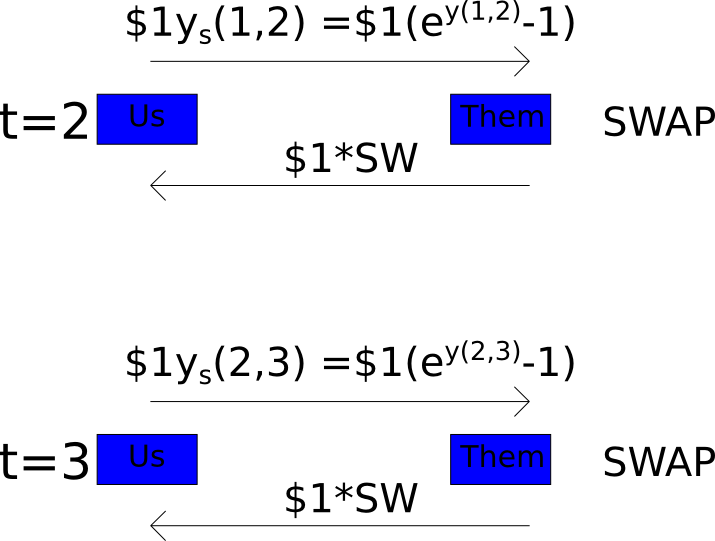
\includegraphics[width=3in]{pics/swap2P.png} \\
  \caption{Swap at $t=2$ and $t=3$}
\label{swap2P}
\end{center}
\end{figure}

Now we have to worry about two floating rates: $y_s(1,2)$ and $y_s(2,3)$. Since we pay the floating rate we need to borrow at the forward rate in $t=1$ and $t=2$ to offset. 

\begin{tiny}
\begin{tabular}{|c|c|c|}
\hline
time & contract/action & cashflow\\
\hline
0 & \begin{tabular}{c}Enter swap to pay $\$1*y_s(t-1,t)$ and receive $\$1*SW$ at $t=2,3$\\ Enter forwards to borrow \$1 at $f(t-1,t)$ for $t=2,3$\\ \end{tabular} & 0\\
\hline
1 & \begin{tabular}{c}Borrow \$1 at $f(1,2)$\\ Lend \$1 at $y(1,2)$ \end{tabular} & 0\\
\hline
2 &\begin{tabular}{c}\\ Borrow \$1 at $f(2,3)$\\ Lend \$1 at $y(2,3)$  \end{tabular}  & \begin{tabular}{c}Pay $\$1\exp(f(1,2))$ from loan\\ Receive $\$1\exp(y(1,2))$ from loan\\ Pay $\$1y_s(1,2)$ on swap \\ Receive $\$1SW$ from swap\\ \end{tabular}\\
\hline
3 & & \begin{tabular}{c}Pay $\$1\exp(f(2,3))$ from loan\\ Receive $\$1\exp(y(2,3))$ from loan\\ Pay $\$1y_s(2,3)$ on swap \\ Receive $\$1SW$ from swap\\ \end{tabular}\\
\hline
\end{tabular}\\
\end{tiny}

The discounted values of all the cashflows are summarised here 

\begin{tiny}
\begin{tabular}{|c|c|c|c|}
\hline
time & value of loans & value of floating & value of fixed\\
\hline
0 & 0 & 0 & 0\\ 
1 & 0 & 0 & 0\\
2 & $e^{-y(0,2)}(\$1e^{y(1,2)}-\$1e^{f(1,2)})$ & $-e^{-y(0,2)}\$1*y_s(1,2) = -e^{-y(0,2)}(\$1*(e^{y(1,2)}-1))$ & $e^{-y(0,2)}*\$1*SW$\\
3 & $e^{-y(0,3)}(\$1e^{y(2,3)}-\$1e^{f(2,3)})$ & $-e^{-y(0,3)}\$1*y_s(2,3) = -e^{-y(0,3)}(\$1*(e^{y(2,3)}-1))$ & $e^{-y(0,3)}*\$1*SW$\\
\hline
\end{tabular}
\end{tiny}

Since these are all in $t=0$ values we can sum up and set equal to zero to find the swap rate:

\[SW | \sum_{\tau=2}^3  e^{-y(0,\tau)}(1-e^{f(\tau-1,\tau)} +SW) = 0 \]

It's a simple matter to find $SW$ that satisfies this equation.

\subsection{The general formula}

The previous example easily generalises to an arbitrary number of periods. For a swap fixing at $t, t+1 \ldots T$ with anniversaries at $t+1,t+2,\ldots,T+1$ the swap price satisfies

\begin{eqnarray}
SW  | \sum_{\tau=t+1}^{T+1}  e^{-y(0,\tau)\tau}(e^{f(\tau-1,\tau)}-1 -SW) = 0  \label{swapprice}
\end{eqnarray}

Notice that since all cashflows are multiples of the notional value we can divide them out  without changing the result. 

This is an intuitive formula. It says \textbf{the sum of discounted differences between the (simple) forward rate and the swap rate should be zero}.

Some swaps pay fixed and floating rates at different times. It's easy to accommodate these. Let $N_F(t)$ and $N_L(t)$ be the fixed and floating notional values. Then 

\begin{eqnarray*}
SW  | \sum_{\tau=t+1}^{T+1}  e^{-y(0,\tau)\tau}N_L(t)(e^{f(\tau-1,\tau)}-1)  - e^{-y(0,\tau)\tau}N_F(t)SW = 0  \label{swapgeneral}
\end{eqnarray*}

We just have to remember to borrow $N_L(t)$ to construct the hedge. With swaps with asyncronous payments sometimes $N_L(t)$ and $N_F(t)$ will be zero. Our formula works fine with this.


\subsection{Worked example: 3 period swap}

\textit{Step 1: Calculate forward rates}\\

Suppose we have the following zero rates:\\
\begin{center}
\begin{tabular}{|c|c|}
  \hline
  % after \\: \hline or \cline{col1-col2} \cline{col3-col4} ...
  $t$ & $y(0,t)$ \\
  \hline
  1&0.05 \\
  2&0.06 \\
  3&0.09 \\
  4&0.08 \\
  5&0.07\\
  \hline
\end{tabular}
\end{center}
We can calculate the forward rates\\
\begin{center}
\begin{tabular}{|c|c|c|}
  \hline
  % after \\: \hline or \cline{col1-col2} \cline{col3-col4} ...
  $t$ & $y(0,t)$ & $f(t,t+1)$ \\
  \hline
  1&0.05 & 0.07\\
  2&0.06 & 0.15\\
  3&0.09 & 0.05 \\
  4&0.08 & 0.03\\
  \hline
\end{tabular}
\end{center}

\textit{Step 2: Construct discounted payoff and solve for swap rate}\\

We can use the general formula

\begin{eqnarray*}
\sum_{\tau=t+1}^{T+1}  e^{-y(0,\tau)}(e^{f(\tau-1,\tau)}-1 -SW) = 0 \\
\Rightarrow e^{-y(0,2)2}(e^{f(1,2)} - 1 - SW) + e^{-y(0,3)3}(e^{f(2,3)} - 1 - SW)+ e^{-y(0,4)4}(e^{f(3,4)} - 1 - SW) =0\\
\Rightarrow e^{-0.06*2}(e^{0.07} - 1 - SW) + e^{-0.09*3}(e^{0.015} - 1 - SW)+ e^{-0.08*4}(e^{0.05} - 1 - SW) =0\\
\Rightarrow SW = 0.094\\
\end{eqnarray*}

So the swap rate is 0.094.

\section{Questions}

\textbf{Question 1:}\\
Calculate the price for a bond that pays a coupon of \$10 per year for 5 years with a \$50 face value if the zero curve is constant at 3\%.

\textbf{Question 2:}\\
If the one year interest rate is $y(1) = 0.02$ and the 5 year interest rate is $y(5) = 0.03$ calculate the 4 year interest rate 1 year forward.

\textbf{Question 3:}\\
Suppose we have the following zero rates:\\
\begin{center}
\begin{tabular}{|c|c|}
  \hline
  % after \\: \hline or \cline{col1-col2} \cline{col3-col4} ...
  $t$ & $y(t)$ \\
  \hline
  1&0.05 \\
  2&0.06 \\
  3&0.07 \\
  4&0.08 \\
  5&0.09\\
  \hline
\end{tabular}
\end{center}


Consider a swap to receive \$1,000,000 times a some fixed swap rate $SW$ each year and pay \$1,000,000 times the one year zero rate $y(t-1,t)$ for four years starting at $t=2$. Calculate the no-arbitrage value of $SW$. (hint: you'll need to use a spreadsheet or mathematical package)



\section*{Appendix: Compounding}


So let's say I borrow \$1 and repay the loan in $t$ years from now with an annual rate of interest $ARI$ paid at the end of each year. I will repay

\[ \$1\underbrace{\left(1+\mbox{ARI}\right)\left(1+\mbox{ARI}\right)\ldots\left(1+\mbox{ARI}\right)}_{\mbox{t times}} \]


or

 \[\$1\left(1+\mbox{ARI}\right)^t \]

Suppose instead that the interest is paid semi-annually. I will now repay \[\$1\left(1+\frac{\mbox{ARI}}{2}\right)^{2t} \]

Suppose instead that the interest is paid quarterly. I will now repay \[\$1\left(1+\frac{\mbox{ARI}}{4}\right)^{4t} \]

Suppose I pay the interest every day. I will now repay \[\$1\left(1+\frac{\mbox{ARI}}{365}\right)^{365t} \]

As the frequency of repayment approaches infinity the repayments will approach \[\lim_{k\rightarrow\infty}\$1\left(1+\frac{\mbox{ARI}}{k}\right)^{kt} = \$1\exp(rt) \]

where $r$ is the \textit{continuously compounded interest rate}.

Say I borrow \$1 with $ARI = 1$ (100\% per year)

\begin{center}
\begin{tabular}{|p{8cm}|p{8cm}|}
  \hline
  % after \\: \hline or \cline{col1-col2} \cline{col3-col4} ...
  k (frequency of repayments) & repayments (one year)  \\
  \hline
  1 & $\$1\left(1+\frac{1}{1}\right)^{1*1} = \$2 $ \\
  4 & $\$1\left(1+\frac{1}{4}\right)^{4*1} = \$2.441406$ \\
  365 & $\$1\left(1+\frac{1}{365}\right)^{365*1} = \$2.714567$\\
  1000 & $\$1\left(1+\frac{1}{1000}\right)^{1000*1*} = \$2.716924 $  \\
  $\infty$ & $\lim_{k\rightarrow\infty}\$1\left(1+\frac{1}{k}\right)^{k*1} = \exp(1*1) \approx \$2.718282$\\
  \hline
\end{tabular}
\end{center}

The number 2.71828182845709... is called $e$. The expression $e^x$ is often written as $\exp(x)$. It is a very important number. If a variable $x$ grows at a rate $g$ for $t$ periods of compounded growth starting at $x(0)$ then its value at time $t$ will be

\[x(t) = x(0)\exp(gt) \]

Back to borrowing. Say I borrow \$1 with $ARI = 0.05$ (5\% per year) for one year
\begin{center}
\begin{tabular}{|p{8cm}|p{8cm}|}
  \hline
  % after \\: \hline or \cline{col1-col2} \cline{col3-col4} ...
  k (frequency of repayments) & repayments (one year) \\
  \hline
  1 & $\$1(1+\frac{0.05}{1})^{1*1} = \$1.05 $  \\
  4 & $\$1(1+\frac{0.05}{4})^{4*1} = \$1.050945$ \\
  365 & $\$1(1+\frac{0.05}{365})^{365*1} = \$1.0512675$ \\
  1000 & $\$1(1+\frac{0.05}{1000})^{1000*1} = \$1.051270 $ \\
  $\infty$ & $\lim_{k\rightarrow\infty}\$1(1+\frac{0.05}{k})^{k*1} = \exp(0.05*1) \approx \$1.051271$\\
  \hline
\end{tabular}
\end{center}

Say I borrow \$1 with $ARI = 0.05$ (5\% per year) for two years
\begin{center}
\begin{tabular}{|p{8cm}|p{8cm}|}
  \hline
  % after \\: \hline or \cline{col1-col2} \cline{col3-col4} ...
  k (frequency of repayments) & repayments (two years) \\
  \hline
  1 & $\$1(1+\frac{0.05}{1})^{1*2} = \$1.1025 $ \\
  4 & $\$1(1+\frac{0.05}{4})^{4*2} = \$1.104486$\\
  365 & $\$1(1+\frac{0.05}{365})^{365*2} = \$1.105163$ \\
  1000 &  $\$1(1+\frac{0.05}{1000})^{1000*2*} = \$1.105168 $  \\
  $\infty$ & $\lim_{k\rightarrow\infty}\$1(1+\frac{0.05}{k})^{k*2} = \exp(0.05*2) \approx \$1.105171$ \\
  \hline
\end{tabular}
\end{center}


We can convert between the $ARI$ and $y$ by comparing a discretely compounded loan with a continuously compounded loan
\begin{eqnarray*}
\mbox{discrete} & =\mbox{continuous}\\
\rightarrow \$1\left(1+\frac{\mbox{ARI}}{k}\right)^{kt} & = \exp(yt)
\end{eqnarray*}
\begin{equation}
\rightarrow y = k \ln \left(1+\frac{\mbox{ARI}}{k} \right)
\end{equation}


So in summary we have:

\textit{Discrete compounding:}

\[FV_{\mbox{discrete}} = \mbox{PV}\left(1+\frac{ARI}{k}\right)^{kt} \]

\textit{Continuous compounding:}

\[FV_{\mbox{continuous}} = \mbox{PV}\exp(yt) \]

We can also use this to discount payoffs which occur in the future by:

\[FV\exp(-yt) = \mbox{PV} \]


\textit{Converting between discrete and continuous compounding:}

\[FV_{\mbox{continuous}} = FV_{\mbox{discrete}} \rightarrow y = k \ln \left(1+\frac{ARI}{k} \right)\]

where
\begin{itemize}
\item PV: present value of loan\\
\item FV: future value of loan\\
\item ARI: annual rate of interest (discrete)\\
\item $k$: number of compounding periods per year\\
\item $t$: number of years\\
\item $y$: continuously compounded interest rate
\end{itemize}






\chapter{Portfolio management }
\section{The Problem}
%Knowledge vs expression intro
We have a portfolio of fixed income securities consisting of \textbf{bonds} and \textbf{swaps}. We want to understand the sensitivity of the portfolio to changes in \textbf{yields}. The \textbf{non-linear} relationship between fixed income security prices and yields, as well as a \textbf{dependence of price on the entire yield} curve makes this task more complicated than a comparable analysis of an equities portfolio. 

The value of a fixed income portfolio is a function of the cash flows due and the yield curves that discount them.  A payment from a different issuer, or due at a different time, will generally be discounted with a different yield curve.

We set two related tasks: 

First, we want a method to \textbf{simulate} the effect of changes in yield curves on a portfolio. If the 30 year treasury yield jumps by 30bps, and the BBB spread widens by 10bps at 2 years and narrows by 10bps at 10 years, we want to know what happens to the value of our portfolio.

Second, we want to be able to \textbf{attribute} changes in portfolio value to different sources. Our portfolio loses 50 million overnight -- we want to know which curve movements caused the damage. 

\section{The relationship between prices and yields }

For each borrower there is a \textbf{yield curve} of interest rates for loans of various maturities. Any bond or swap can be priced completely given the appropriate curve.

\textbf{Example: a bond} A government bond pays a 10\% coupon in one year and the face value (\$100) in two years time. The yield curve is $y(1)= 0.04$, $y(2) = 0.06$. 


The price of the bond is calculated by discounting the two cash flows (the coupon and the face value) by the appropriate yield. 

\begin{eqnarray*}
\textrm{Bond price} = \underbrace{10 \exp(-y(1)*1)}_{\textrm{Discount coupon at $y(1)$}} + \underbrace{100\exp(-y(2)*2)}_{\textrm{Discount face value at $y(2)$}}\\
=10 \exp(-0.04*1) + 100\exp(-0.06*2) = 98.3
\end{eqnarray*}

\begin{figure}[htbp]
\begin{center}
  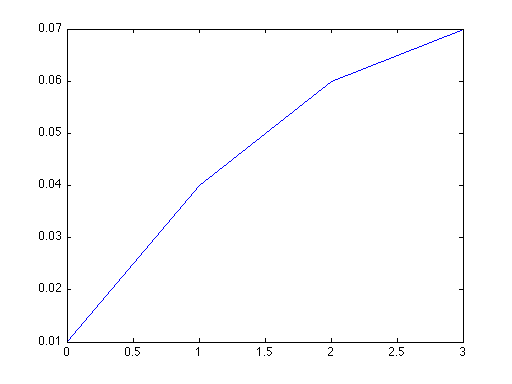
\includegraphics[width=3in]{pics/simpleYieldCurve.png} \\
  \caption{Yield curve with $y(1) = 0.04$, $y(2)=0.06$, $y(3)=0.07$}
\label{frArb}
\end{center}
\end{figure}

\textbf{Example: A swap} A swap receives the previous year's government rate $y(t-1,t)$ at $t=2,3$ and pays a fixed swap. The yield curve is $y(1) = 0.04$, $y(2) = 0.06$, and $y(3) = 0.07$. The notional value of the swap is 1 million.

The swap is priced to make the fixed and floating sides present value to zero. . The current value of the swap is the value of all remaining fixed and floating payments. This is:

\[V_{\textrm{swap}} = \sum_{\tau=2}^{3}  e^{-y(0,\tau)\tau}1M(e^{f(\tau-1,\tau)}-1 -SW) \]
 
The forward rates are

\[ f(1,2) = \frac{y(2)*2-y(1)*1}{2-1} = 0.08 \]  

\[ f(2,3) = \frac{y(3)*3-y(2)*2}{3-2} = 0.09 \]

The fair value for the swap rate is 0.088480, which is completely determined by the zero rates $y(0,t)$
%(We could also look at futures on bonds, forward rate agreements, options and so forth)


\section{Sensitivity: duration, convexity, and beyond}
How do changes in the yield curve change the value of our portfolio?

The answer depends on what kind of a change occurs in the yield curve. If all the rates on the yield curve move the same amount up or down the same amount the sensitivity will be easily described by a single number. However it's more likely that some rates will move more than others. We'll start with the simple case where everything moves the same.

\subsection{Parallel shifts in the yield curve}

Define the value of a bond as the discounted sum of cashflows

\[V = \sum_i CF_i e^{-y(t_i)t_i} \]

Now let the yield at $t_i$ be decomposed into a base yield $\bar{y}$ and an adjustment $\alpha_i$

\[V = \sum_i CF_i e^{-(\bar{y}+\alpha_i)t_i} \]

The sensitivity of the price to a simultaneous change in all the yields by the same amount is

\[ \frac{\partial V}{\partial \bar{y}} = \sum_i -t_i CF_i e^{-(\bar{y}+\alpha_i)t_i} \]

Expressing this as a percentage of value and changing the sign is 

\begin{eqnarray*}
 -\frac{1}{V}  \frac{\partial V}{\partial \bar{y}} = \frac{1}{V} \sum_i t_i CF_i e^{-y(t_i)t_i} 
 \end{eqnarray*}

This number is sometimes called the \textbf{modified duration} of the bond. Modified duration has a remarkable secondary interpretation: it's the \textbf{time weighted sum of the cashflows}.  If you imagine all the discounted cashflows on a plank representing time the this number is the location of the pivot (in time) that would make the plank balance exactly. 

\begin{figure}[htbp]
\begin{center}
  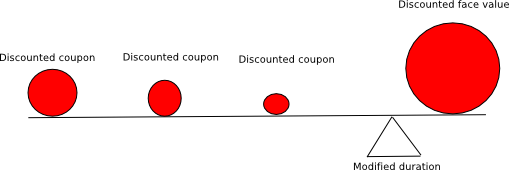
\includegraphics[width=3in]{pics/modDurn.png} \\
  \caption{Duration is the balance point of the discounted cash-flows}
\label{modDurn}
\end{center}
\end{figure}

For a zero coupon bond this is exactly equal to the maturity:

 \[-\frac{1}{V}  \frac{\partial V}{\partial \bar{y}}  = \frac{t CF e^{-y(t)t}}{CF e^{-y(t)t}} = t \]
 
 For a non-zero coupon bond this will be somewhat less than the maturity. 
 
\begin{figure}[htbp]
\begin{center}
  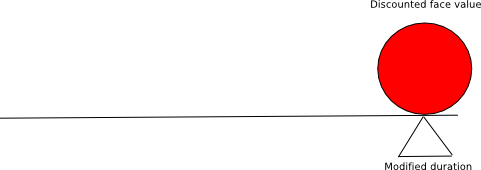
\includegraphics[width=3in]{pics/modDurnZc.png} \\
  \caption{Modified duration of a zero coupon bond is the maturity }
\label{modDurnZc}
\end{center}
\end{figure}
 
Duration is useful because it gives a sense of how large a move in the price of the bond will arise from a shift in yields. If the yield curve shifts up by 1\% the price of a 2 year treasury bond will not move much, the price of a 30 year treasury bond will move drastically. 

Duration is also \textit{additive} over a portfolio. We can add up all durations of each security in the portfolio to get the total first order sensitivity. 

The problem with duration is that it only answers a very specific question: ``what happens to the price of a bond when the yield curve shifts uniformly?" The number is a summary of the effects of each yield on each cashflow of the bond. We could get an better picture by looking at the effect of changes at any point on the curve. Duration is a useful summary, but it can only ever be an approximate measure of interest rate sensitivity.  


\textbf{Example: Duration of a bond}
Returning to the simple bond of the previous example, and with the same yield curve, the duration is

\[ \frac{1*10 \exp(-0.04*1) + 2*100\exp(-0.06*2)}{98.3} = 1.9023  \] 

The \textbf{dollar duration} is the same but without dividing by the bond price

\begin{eqnarray*}
\frac{\partial V}{\partial \bar{y}} = \sum_i -t_i CF_i e^{-(\bar{y}+\alpha_i)t_i}\\
  = -1*10 \exp(-0.04*1) + -2*100\exp(-0.06*2) = -1.87 
 \end{eqnarray*}

This means the price of the bond will change by approximately  \$1.87  for a 0.01 move in the interest rate. This is approximate because the price is not a linear function of the yield, so the duration will itself change with the yield. The change is larger if the yield curve is lower.

We can trace out the change in sensitivity for a range of yield curves:

\begin{center}
\begin{tabular}{|c|c|c|c|}
\hline
$y(1)$ & $y(2)$ & duration & dollar duration\\
\hline
0.02& 0.04 & 1.904 &-1.94\\
0.03 & 0.04 &1.903 &-1.91\\
\textbf{0.04} & \textbf{0.06} & \textbf{1.902} & \textbf{-1.87} \\
0.05 & 0.07 & 1.901&-1.83\\
0.06 & 0.08 & 1.900 &-1.8\\
\hline
\end{tabular}
\end{center}

\textbf{Example: Duration of a swap}
Consider again the swap from the earlier example. Swap duration involves two complications. First, since the swap is priced correctly it has no `value' as would a bond, so it is impossible to divide by $V$ in the usual duration calculation. We must therefore use \textbf{dollar duration}. Second, the value of the floating cashflows are valued using forward rates, and so are also sensitive to movements in the yield curve. Normal bonds don't have this problem because all cashflows are fixed.

It's not a huge problem. All we do is note that each cashflow $CF_i$ of the swap is now also a function of the \textit{level} of yields $\bar{y}$. 

\[V_{\textrm{swap}} = \sum_i CF_i(\bar{y}) e^{-y(t_i)t_i} \]

The dollar duration is then given by the product rule

\begin{eqnarray*}
\frac{\partial V}{\partial \bar{y}}  =  \sum_i -t_i CF_i(\bar{y}) e^{-y(t_i)t_i} + \frac{\partial CF_i(\bar{y})}{\partial \bar{y}} e^{-y(t_i)t_i} \\
\end{eqnarray*}

Recall that the arbitrage free price of the cashflow is 

\[CF_i = N(e^{f(t_i-1,t_i)}-1-SW)  \]

Where $N$ is the notional value and $SW$ is the swap rate. The one period forward price has the same sensitivity to to $\bar{y}$ as any zero rate so the duration of the swap is

\begin{eqnarray*}
 \frac{\partial V_{\textrm{swap}}}{\partial \bar{y}}  = \sum_i -t_i N(e^{f(t_i-1,t_i)}-1-SW) e^{-y(t_i)t_i} + e^{f(t_i-1,t)} e^{-y(t_i)t_i} \\
 = -2*1M (e^{f(1,2)}-1-SW )e^{-y(2)*2} +  e^{f(1,2)}e^{-y(2)*2}  +\\
  -3*1M (e^{f(2,3)}-1-SW )e^{-y(3)*3} +  e^{f(2,3)}e^{-y(3)*3} \\ 
 = -2*1M (e^{0.08}-1-0.0885 )e^{-0.06*2} +  e^{0.08}e^{-0.06*2}  +\\
  -3*1M (e^{0.09}-1-0.0885 )e^{-0.07*3} +  e^{0.09}e^{-0.07*3} \\ 
 = 4635.5\\
\end{eqnarray*}

So, approximately, a 0.1\% upward shift in all yields will cost the swap-holder \$46.36. 

\subsection{Second order sensitivities and other measures}
Most fixed income securities do not have a linear payoff in yield: the duration changes as the yields change. Also yield curves rarely shift in neat parallel movements. To get a broader picture we need higher order sensitivities.

The second order sensitivity is called the \textbf{convexity}. If the cashflows are not a function of the yield this is

\[ \frac{\partial^2 V}{(\partial \bar{y})^2} =  \sum_i t_i^2 CF_i e^{-y(t_i)t_i}  \] 
 
 If cashflows are a function of yields (as with a vanilla swap) we have
 
 \[\frac{\partial V}{\partial \bar{y}}  =  \sum_i -t_i CF_i e^{-y(t_i)t_i} + \frac{\partial CF_i(\bar{y})}{\partial \bar{y}} e^{-y(t_i)t_i} \]
 
 so
 
  \[\frac{\partial^2 V}{(\partial \bar{y})^2}  =  \sum_i t_i^2 CF_i e^{-y(t_i)t_i} + \frac{\partial^2 CF_i(\bar{y})}{(\partial \bar{y})^2} e^{-y(t_i)t_i} - t_i\frac{\partial CF_i}{\partial \bar{y}}e^{-y(t_i)t_i} \]


This is the \textbf{dollar convexity}. If we want to express the convexity as a proportion of the price we can divide by $V$. Convexity is a useful measure as it shows how quickly the duration is changing. A portfolio with high convexity can be very risky as portfolio sensitivities can quickly accelerate.


\section{Simulation and attribution}

\subsection{Breaking it down}
Fixed income portfolios will typically have a number of bonds (and swaps and futures and options) from various issuers and at various maturities. As yield curves shift the value of the portfolio changes.  \textbf{Attribution} is the process of decomposing the sources of these changes in price.

The purpose of the process is to gain an insight into where our returns are coming from. If we make \$20 on our portfolio we want to know how much of that is due to changes in the 10 year treasury yield, and how much due to the change in the 2 year BBB spread on treasuries. 

A sensible way to do this is to break down the zero rate on each issuer into a number of components. For example the two year zero rate for a particular BBB issuer is the 2 year government rate plus the 2 year credit spread. 

\begin{figure}[htbp]
\begin{center}
  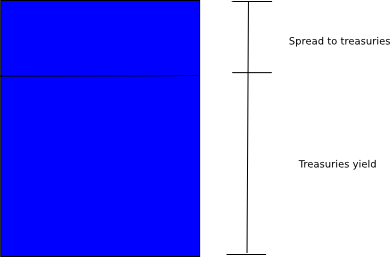
\includegraphics[width=3in]{pics/yCurveDec1.png} \\
  \caption{Yield = treasuries yield + spread}
\label{yCurveDec1}
\end{center}
\end{figure}

We can drill down further if we like: the two year government rate is the real rate plus inflation. (If there is a market for inflation swaps we can know this exactly). The credit spread for a particular BBB issuer is the BBB reference rate plus or minus the spread for that issuer against the reference rate. 

\begin{figure}[htbp]
\begin{center}
  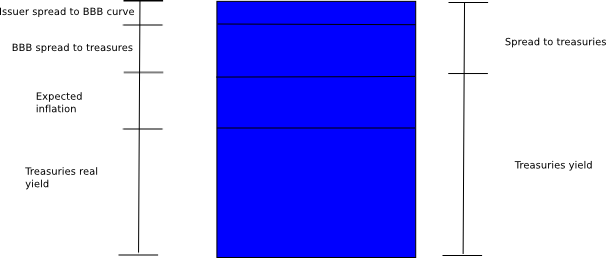
\includegraphics[width=3in]{pics/yCurveDec2.png} \\
  \caption{Yield = treasuries yield + spread = treasuries real yield + expected inflation + BBB spread to treasuries + issuer spread to BBB}
\label{yCurveDec1}
\end{center}
\end{figure}

For an issuer $a$, $y_a(t)$ is the zero rate for maturity $t$. The return to a portfolio can be approximately broken down to the changes in each of these components, as well as the passage of time.

\[y_a(t) = y_{\textrm{real treasury yield}}(t) + y_{\textrm{inflation}}(t) + y_{\textrm{reference yield for issuer $a$}}(t) + y_{\textrm{spread of issuer $a$ to reference yield}}(t)\]

Or any other decomposition of interest. 


\subsection{First principles or perturbation?}
For a given change in all the components of each zero rate $y_a(t)$ to a new curve $y_a'(t)$ we can determine the change in the value of a portfolio by comparing the value of each cashflow at the old yield and new yield. The sum of these changes will be the total change in the value of a the portfolio. 

\[ V = \sum_a \sum_i CF_i^a \exp(-y_a(t)t)\]

So for a change in a particular yield $y_a(t)$ to $y_a^{'}(t)$ 

\[ \Delta V = \sum_a \sum_i CF_i^a \exp(-y_a(t)t) - \sum_a \sum_i CF_i^a \exp(-y_a'(t)t)  \]

We then sum over all $a$ to give the total portfolio change. We can also divide up the yield into its components and trace the change in portfolio value due to each yield change. This is called the \textbf{first principles} approach.

Alternatively we can take a Taylor series expansion for each yield

\[ \Delta V = \frac{\partial V}{\partial y_a(t)}  (y_a(t)-y_a'(t)) + \frac{1}{2}\frac{\partial^2 V}{\partial y_a(t)^2} (y_a(t)-y_a'(t))^2 + O((y_a(t)-y_a'(t))^3) \]

(where $O((y_a(t)-y_a'(t))^3)$ denotes a series of terms that are at most of order $(y_a(t)-y_a'(t))^3$ -- namely quite small so we ignore them)

This is called the \textbf{perturbation} approach.

The advantage of the perturbation approach is that it allows us to express the change in value in terms of duration and convexity without worrying about every cash flow. This gives a very compact (though slightly approximate due to removing higher order terms) summary of the sensitivity of the portfolio to changes in particular yields, or to parallel shifts in any of the curves.

\textbf{Attribution example}

Let's say we have a portfolio of 1 treasury bond and 1 corporate bond issued by B-Corp. Both bonds have a maturity of two years, a face value of \$100, and pay a 10\% coupon after 1 year. 

We have two relevant yield curves: the treasury curve, and the B-Corp curve. It is useful to think of the B-Corp curve as a spread to treasuries (the additional yield on B-corp debt over same maturity treasury debt). Suppose the curves are initially thus:

\begin{tabular}{|c|c|c|}
\hline
 Period & 1 & 2\\
 \hline
Treasury & 0.03 & 0.03\\
B-Corp spread to treasuries & 0.03 & 0.03\\
\hline
\end{tabular}

The total yield on 1 year B-Corp shares is then the rate on treasuries plus the spread (0.03+0.03 = 0.06). We can price the portfolio by the discounted cash flows:

\[ V = \underbrace{10 \exp(-0.03*1)+ 100 \exp(-0.03*2)}_{\textrm{Treasury bond}} + \underbrace{10\exp(-0.06*1)+ 100 \exp(-0.06*2)}_{\textrm{B-Corp bond}} = 201.99\]

 All at once the treasury yield curve shifts up by 100bps, as does the B-Corp credit spread. 

\begin{tabular}{|c|c|c|}
\hline
 & 1 & 2\\
 \hline
Treasury & 0.04 & 0.04\\
B-Corp spread to treasuries & 0.04 & 0.04\\
\hline
\end{tabular}

The revised portfolio price is 

\[ V = \underbrace{10 \exp(-0.04*1)+ 100 \exp(-0.04*2)}_{\textrm{Treasury bond}} + \underbrace{10\exp(-0.08*1)+ 100 \exp(-0.08*2)}_{\textrm{B-Corp bond}} = 196.37\]

The portfolio value has decreased by \$5.63. How does this break down?

Using the first principles approach we can price each cash flow under the old ($y$) and new ($y'$) yield curves. 

\begin{tiny}
\begin{tabular}{|c|cc|c|cc|c|}
\hline
 & & y&  & & y' & \\
 Maturity & 1 & 2 & $\Sigma$ & 1 & 2 & $\Sigma$ \\
 \hline
Treasury bond & $10e^{-0.03*1} = 9.70$  & $100e^{-0.03*2}=94.18$ & 103.88 & $10e^{-0.04*1} = 9.61$ & $100e^{-0.04*2}=92.31$ & 101.92\\
B-Corp Bond & $10e^{-0.06*1} = 9.42$ & $100e^{-0.06*2}= 88.69$ & 98.11 & $10e^{-0.08*1}=9.23$ & $100e^{-0.08*2}=85.21$ & 94.45\\
\hline
 & & & 201.99 & & & 196.37\\
 \hline
\end{tabular}
\end{tiny}

Under the first yield curve the portfolio is worth  103.88 + 98.11 = 201.99.  Under the second the portfolio is worth 101.92+ 94.45 =196.37 . The difference is 5.62 (we accumulated -0.01 due to rounding). 

How much of this is due to the shift in the treasuries curve and how much to the shift in the B-Corp curve? The surprising answer is that it depends which way you look at it. 

Let's say the treasury curve shifts first from $y(1) = y(2) = 0.03$ to $y(1) = y(2) = 0.04$. This pushes the B-Corp curve from $y(1) = y(2) = 0.06$ to $y(1) = y(2) = 0.07$. Then the shift in B-Corp spread pushes the B-Corp curve to $y(1) = y(2) = 0.08$.

If the B-Corp spread moves first then the B-Corp curves moves from $y(1) = y(2) = 0.06$ to $y(1) = y(2) = 0.07$. The shift in treasuries moves it up to $y(1) = y(2) = 0.07$ to $y(1) = y(2) = 0.08$.

In both cases the treasury is first worth 103.88 and then 101.92 (a change of -1.96).  However in the first case the treasuries shift decreases the price of the B-Corp bond from 98.11 to 96.25 (a change of -1.85); and in the second case from 96.25 to 94.45 (a change of -1.81). The difference is due to the convexity of the bond. The sensitivity to a 100bps shift in yields is lower after a shift has already occurred.

At still higher prevailing levels of B-Corp yields the difference would be smaller still as we see in the table below.

\begin{tabular}{|c|c|}
\hline
level of B-Corp yields & change in B-Corp bond price after 1\% increase in yields\\
\hline
0.06 & -1.85\\
0.07 & -1.81\\
0.08 & -1.78\\
0.09 & -1.74\\
0.1 & -1.71\\
\hline
\end{tabular}


The 4 cent difference might seem like small beans but for larger yield moves and at longer maturities these differences become significant. In practice attribution must simply follow a convention: For instance we might measure the impact of the treasury curve first and the B-Corp spread afterwards.

Now let's try the perturbation approach. Recall that we can approximate the change in value arising from changes in yields by the first two terms of the Taylor series.

\[ \Delta V \simeq \frac{\partial V}{\partial y_a(t)}  (y_a(t)-y_a'(t)) + \frac{1}{2}\frac{\partial^2 V}{\partial y_a(t)^2} (y_a(t)-y_a'(t))^2  \]

The relevant terms for both bonds in each period are below:

\begin{tabular}{|c|cc|cc|}
\hline
 Issuer & &  Government bond & & B-Corp\\
 Period & 1 & 2 & 1 & 2\\
 \hline
 $\frac{\partial V}{\partial y(t)}$ & -9.70 & -188.35 & -9.42 & -177.38\\
 $\frac{\partial^2 V}{\partial y(t)^2}$& 9.70 & 376.71& 9.42 & 354.77\\
 $\Delta y(t)$ & 0.01 & 0.01 & 0.02 & 0.02\\
 $(\Delta y(t))^2$  & 0.001 & 0.001 & 0.004 & 0.004\\
 $\Delta V \simeq \frac{\partial V}{\partial y(t)} + \frac{1}{2} \frac{\partial^2 V}{\partial y(t)^2}(\Delta y(t))^2$ & -0.0966 & -1.8647 &  -0.1865 & -3.4767\\
 \hline
 \end{tabular}

From this we can see the total anticipated change in the government bond price is -0.0966 -1.8647 = -1.9613, and the anticipated change in the B-Corp bond is   -0.1865 -3.4767 = -3.6632. Both are around what we expect.

The table also shows us the effect of the price from movements in different parts of the curve. The value of the \$10 coupon on the government bond moves -0.0966 due to a 0.01 increase in y(1); the value of the \$100 at maturity moves -1.8647 due to the 0.01 increase in y(2). 

This table allows us to estimate other changes too. By changing the row with $\Delta y(t)$  we can accommodate any change in the structure of the yield curve.

We still have the question of how much of the change is due to the change in the government curve and how much to the change in the B-Corp spread. Again the answer depends which change we consider first. One approach is to consider more `primitive' moves first: we consider a change in the government rate before a change in the BBB reference rate; and  that before a change in the B-Corp spread to the reference rate.

Reality is more complicated than this simple example. Bonds pay irregular coupons; not all points on the yield curve are available or reliable; some bonds embed options for early repayment, which complicates matters. There are other complexities too. But the basic process is quite simple. We have a series of zero curves which can be used to price known future cash flows. As the curves move the cashflows must be repriced. Sensitivities change. The rest is detail.

%Higher order Taylor series and Taylor series involving time.\\ An integral representation \\Appendix on Taylor series?

\section{A general schema for fixed income portfolio management}

Take a step back. We know a few things:

\begin{enumerate}
\item  Every potential borrower (including you and I) has a yield curve giving the market interest rate of loans at all maturities. 
\item Each of these rates can be decomposed into a risk free part (proxied by government rates) and a credit part (the difference between each rate and government rate). We can break rates down further by splitting government rates into real rates and expected inflation, and credit spreads into reference rates for certain classes of credit and spreads to those reference rates. Or any other decomposition of interest.  
\item Each fixed income security is a series of cashflows due at some future time. The value of those cashflows is determined by discounting them by the rate (yield) for that issuer at that maturity.
\item When yield curves shift the value of these discounted cashflows change. We can \textbf{attribute} these changes by  recalculating the value of the securities at the old and new yields. Because different yield curves have common components we can vary the components one at a time, and observe how much each change affects the value 
\item We follow the same process to determine the effect of hypothetical changes in yield curves\\
\item The total effect of a change in yields can be well estimated by the first two terms in a Taylor series of the value of a each cashflow as a function of its yield.
\end{enumerate}

A general representation of a fixed income portfolio is then 

\begin{eqnarray*}
V = \sum_a \int CF_a(t)e^{-y_a(t)t}dt \\
y_a(t) = \omega_a' c(t)
\end{eqnarray*}

Where $CF_a(t)$ is a cashflow from issuer (borrower) $a$ in period $t$ and $y_a(t)$ is the yield for issuer $a$ for loans with maturity $t$. 

We decompose $y_a(t) = \omega_a' c(t)$ where $c(t)$ is a vector of component yields and $\omega_a$ is a vector of weights of each of the component yields for issuer $a$. This allows us to calculate the effect of each component yield on the total portfolio. For most cases the components of $c(t)$ will be \textbf{orthogonal} so $\frac{\partial c_i(t)}{\partial c_j(t)} = 0$ for $i \neq j$.  

For example if the compenents were 

\[c(t) = (y_{\textrm{treasuries}}(t),y_{\textrm{B-Corp spread to treasuries}}(t))\] 

Then weight vector for treasury bonds would be $\omega_{\textrm{treasures}} = [1, 0]$, and for B-Corp bonds $\omega_{\textrm{B-Corp bonds}} = [1,1]$.

We can derive all first and second order sensitivities easily. The results are for fixed cashflows. Extending to cases where the cashflow is a function of yields (for instance if swaps are involved) is straightforward but a little messier.

\begin{eqnarray*}
\frac{\partial V}{\partial y_a(t)} = \sum_a -t CF_a(t) e^{-y_a(t)t}\\
\frac{\partial^2 V}{\partial y_a(t)^2} = \sum_a t^2 CF_a(t) e^{-y_a(t)t}\\
\frac{\partial V}{\partial c_i(t)} = \sum_a -\omega_a(i) t CF_a(t) e^{-y_a(t)t}\\
\frac{\partial^2 V}{\partial c_i(t)^2} = \sum_a \omega_a(i)^2t^2 CF_a(t) e^{-y_a(t)t}
\end{eqnarray*}

Sensitivities to the \textbf{levels} of individual yield curves $y_a(t)$ or to the \textbf{components} $c_i(t)$ (call these $\bar{y_a}$ and $\bar{c_i}$) are straightforward:

\begin{eqnarray*}
\frac{\partial V}{\partial \bar{y_a}} = \int_0^{\infty}\frac{\partial V}{\partial y_a(t)}dt\\
\frac{\partial^2 V}{\partial \bar{y_a}^2} = \int_0^{\infty}\frac{\partial^2 V}{\partial y_a(t)^2}dt\\
\frac{\partial V}{\partial \bar{c_i}} = \int_0^{\infty}\frac{\partial V}{\partial c_i(t)}dt\\
\frac{\partial^2 V}{\partial \bar{c_i}^2} = \int_0^{\infty}\frac{\partial^2 V}{\partial c_i(t)^2}dt\\
\end{eqnarray*}


\section{Questions}

\textbf{Question 1}\\

A bond pays a \$5 coupon at $t=0.5$ and a \$100 coupon at $t=50$. Yields are $y(0.5) = 0.01$ and $y(50) = 0.02$.

\begin{tabular}{l}
(a) What is the modified duration and convexity of the bond?\\
(b) What is the dollar duration of a:\\
\begin{tabular}{l}
(i)  100bps downward shift in the yield curve\\
(ii) 100bps downward movement in y(0.5)\\
(iii) 100bps downward movement in y(50)\\
\end{tabular}\\
(c) Calculate the expected change in price from using a first principles approach and a Taylor series approximation.
\end{tabular}

\medskip

\textbf{Question 2}\\

Say the yield curve is  $y(0.5) = 0.01$, $y(1) = 0.01$, $y(50) = 0.02$, $y(51) = 0.02$

The sway pays y(0.5,1)*1M at $t=1$ and $y(50,51)*1M$ at t=51 and receives a fixed swap rate.

\begin{tabular}{l}
(a) What is the appropriate swap rate?\\
(b) What is the dollar duration of the swap?\\
\end{tabular}

\medskip

\textbf{Question 3}\\

Reconsider the bond in question 1. This bond is issued by B-Corp. B-Corp yields can be decomposed into a treasuries component and a spread. Say the curves move as in the table below. How much of the change in yields can be attributed to the change in the treasuries curve and how much to the change in the B-Corp spread?


\begin{tabular}{|c|c|c|c|c|}
\hline
 & & y&  & y'  \\
 Maturity & 0.5 & 50 & 0.5 & 50 \\
 \hline
Treasury bond (bps) & 75 & 150 & -25 & 100 \\
B-Corp spread (bps) & 25 & 50 & 25 & 0\\   
 \hline
\end{tabular}
%\end{block}



%Contract specifications
%Pricing
%Decomposing yields (inflation/credit/etc)
%Duration of a bond future/option




\chapter{Trading}


\section{The problem}

Imagine you have a big pot of money that you decide to lend out. There are two basic things you need to decide:

\begin{enumerate}
\item The maturity of the loans (how long you lend the money out for)
\item The riskiness of the borrowers
\end{enumerate}

The first is the \textbf{duration objective}, the second is the \textbf{credit objective}. Most  fixed income trading is in service of one of these. 

There are other important objectives such as exposure to particular currencies or inflation. These are important, but they are not core fixed income as they don't relate to the actual loans. 

Many different instruments and trading techniques are used to pursue these objectives. A major decision is whether to trade using \textbf{cash instruments} (claims to actual loans) or \textbf{derivatives} like forwards and swaps. Often the same objective can be pursued through both, but in different ways. There is a strong argument to use derivatives wherever possible, basically because it's cheaper.

The differences can be subtle and sometimes very difficult to quantify, largely due to the \textbf{non-linearities} inherent in fixed income instruments. This makes some aspects of fixed income trading more art than science. But it also makes it a richer and more textured landscape on which to paint the image of your portfolio preferences.

We'll proceed in four courses: first an aperitif of notation, and summaries of instruments, and processes; then a main course of duration and credit trading served with a side of popular carry and rolldown strategies. And for desert: inflation and currency.  If you're still hungry after that you might enjoy the appendix on credit instruments and pricing.


\section{Preliminaries}

\subsection{Notation}

\begin{itemize}
\item $AT$ - bond from issuer $A$ with maturity $T$
\item Zero coupon price: $P_{AT}^{FV}(t)$  -- price of a bond with a face value of \$FV from issuer $A$ with maturity $T$ at time $t$.
\item Zero coupon yield: $y(T1,T2)$  --yield on loan starting at $T1$ and maturing at $T2$ determined at $T1$
\item Zero coupon yield for a particular bond: $y_{AT}$ -- yield on the $AT$ bond
\item Zero coupon forward yield: $f(T1,T2)$ -- yield on loan starting at $T1$ and maturing at $T2$ determined now.
\item Swap: $SW_{AT_1,BT_2}$ -- self financed swap paying some amount of $AT_1$ and receiving one $AT_2$
\item Portfolio value: $V(t)$ -- value of some portfolio at time $t$
\end{itemize}

Unless otherwise specified all prices are for zero coupon bonds at $t=0$.

\subsection{Instruments}

\subsubsection{Bonds}

 A bond is a series of cashflows promised at different times in the future. A common structure is to have a final payment called the \textbf{face value} and regular payments called \textbf{coupons} as a percentage of face value. Some bonds have uncertain (\textbf{floating}) future payments. The price of a bond is the discounted value of all the payments.  Each payment should be discounted at the \textbf{zero coupon bond yield} for that maturity.

\subsubsection{Swaps}

A \textbf{swap} is any arrangement which swaps one series of cashflows for another. Since a series of cashflows is valued as a \textbf{bond}, a swap can be viewed as an exchange of bonds, or of a series of bonds. Often swaps are specified in terms of a \textbf{notional value}, with cashflows being either a \textbf{fixed rate} or a \textbf{floating rate} of the notional value with some regularity. For example a swap might swap the 3 month government rate for a fixed 4\% on a notional value of \$1M with payments each year. 


\subsubsection{Rates futures and forward rate agreements}
Bonds and swaps have a non-linear exposure to future interest rates. A \textbf{rate future} contract (sometimes called a \textbf{forward rate agreement}) is a linear exposure to rates at some point in future. For example a futures contract might be to pay \$100 times the three month interest rate in 9 months time. These provide a similar payoff to a certain type of interest rate swap, except that rates futures provide a payoff linear in the future rate where swaps are usually convex.

%For most simple bets on rates rate futures are an easy way to implement a particular view. For most of the examples below we won't use them because arbitrage the arbitrage argument is a little tricky. Using swaps gives us a clearer arbitrage argument so we can understand what's going on in the transaction. However for most purposes if you want to punt on interest rates or the shape of the curve rates futures are the way to go. 

\subsection{Processes}

\subsubsection{Repos}

It is possible to short sell bonds through \textbf{repurchase agreements} or \textbf{repos}. A repo is a borrowing agreement. We borrow a bond and agree to give it back later. Why do we do this? Because we immediately sell the bond for cash and \textbf{repurchase} it later when the loan is due.

If we have a riskless zero coupon bond with a face value of \$1 and two year maturity the short sale is like this:


\begin{center}
\begin{tabular}{|c|c|}
\hline
t=0 & Borrow bond \\
t=0 & Sell bond at market price for $P_{2}(0)$ cash  \\
       & (invest in a one year bond)\\
\hline
t=1 & Buy bond back at market price $P_2(1)$ \\
t=1 & Give bond back to lender\\
\hline
\end{tabular}
\end{center}

At $t=1$ the transaction is the risk free return on the repo cash less the cost to repurchase the bond: 

\[ V(1) =  \underbrace{P_2(0)\exp(y(0,1))}_{\textrm{risk free return}} - \underbrace{P_2(1)}_{\textrm{cost to repurchase loan}} \]

This generates the opposite return to short selling the one year bond to buy the two year bond. We do it to get a negative exposure to the price (and positive exposure to the yield). In this way we can use bonds to bet on future interest rates. The payoffs $V(1)$ as a function of price and yield is in figure \ref{fig:repo}.


\begin{figure}[ht]
\centering

\subfigure[As a function of price]{
   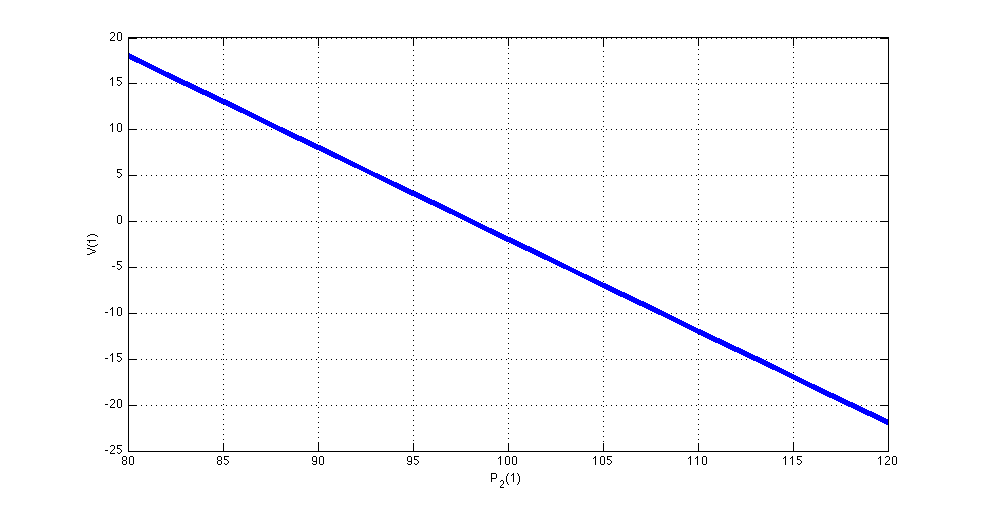
\includegraphics[width=3in] {pics/repoP}
   \label{fig:repoP}
 }

 \subfigure[As a function of future yield]{
   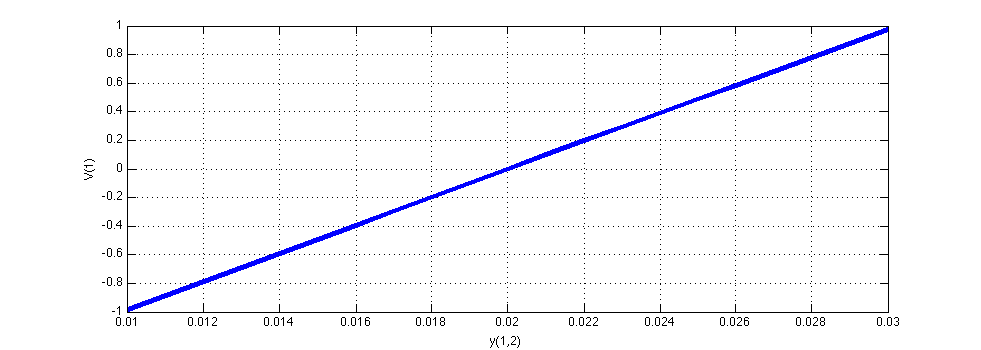
\includegraphics[width=3in] {pics/repoR}
   \label{fig:repoR}
 }
\caption{$V(1)$ for repurchase agreement}
\label{fig:repo}
\end{figure}


%set asset repo as exercise. 
 
%There's a deeper point here. All assets are bought with other assets and so all yields must be contrasted with the yields of alternative assets. This is visible when we do a short sale because we have to reacquire the repo at a different price, but it is nonetheless a real cost. If I borrow (short sell) money to buy a house I want the house to appreciate more than a money asset.\footnote{adjusted for the value the house provides} But if I start with \$100 and leave it in cash I am still \textit{short} houses even though I don't have a repurchase agreement.

%We've assumed that the bond is riskless so why would anybody be willing to loan the bond to you or me for no extra? It's true that they end up in the same position but that's only if we don't scamper off with the bond. In the real world repos are costly but not as much as you would think.

Aren't we forgetting something? Shouldn't there be an interest rate on the repo? The surprising answer is ``no".  The reason is that whoever lends the bond doesn't lose anything provided that the bond is repaid. Since they don't lose anything they should be satisfied with a token payment close to zero for the loan plus something for the credit risk. The credit risk approaches zero if the contract has sufficient collateral and is well margined.

\subsubsection{Collateral and margining} 

The easiest way to reduce credit risk on a repo is to provide a large amount of collateral. If there is a sufficiently large buffer between the value of the loan and the saleable value of the collateral the loan becomes riskless.

Home loans are a good example. A home loan is a repo (short selling a bond) and a long position in an asset. The loan (repo) is collateralised with the asset: if you stop paying your mortgage the bank will sell your house. If the value of the house is always more than the value of the loan they can't lose. The same principle applies to other repos. If you provide a sufficiently valuable asset as collateral the repo rate will approach zero.\footnote{This isn't true if the asset pays any income like coupons or dividends over the course of the repo. If it does the repo rate will include the discounted value of these payments.}

A clever technique for collateralising a repo is \textbf{margining}. Margining is when you give a little bit of collateral initially but demand more (in a \textbf{margin call}) if the asset price moves adversely. If the price changes are small relative to the margin there's no credit risk because the contract can be closed if fail to pay a margin call. 

\textbf{Example: margining}
Say I enter a futures contract to buy a tonne of corn in a year's time for \$100. I put up 10\% of the price as margin.  The futures price moves to \$105 so I have to provide an additional \$5 in margin to keep the 10\% buffer. If I don't provide the margin the futures seller closes out the contract an reenters with another buyer. As long as the margin is large enough to cover market moves there is no credit risk. After a year the contract can settle in cash because the accumulated margins will equal the difference between the contracted futures price and the spot price at expiry.

\subsubsection{Self financed portfolios}

Say you have two zero coupon bonds: $AT_1$ and $BT_2$. We can construct a portfolio by repoing (short selling) a certain amount of the first bond to finance the purchase of one of the second bond. 

To buy one $BT_2$ we need to repo  $P_{BT_2}(0)/P_{AT_1}(0)$ of the $AT_1$s. The total portfolio value is

\[V(0) =  -\frac{P_{BT_2}(0)}{P_{AT_1}(0)}*P_{AT_1}(0) + P_{BT_2}(0) = 0 \]

after $T1<T2$ the value first bond has matured and repays FV (face value) so the value is

\[V(T1) = -\frac{P_{BT_2}(0)}{P_{A_T1}(0)}*FV + P_{BT_2}(T1)   \]

If the face value is a constant the only uncertain value is $P_{BT_2}(T1)$. In summary this portfolio costs zero upfront and is a linear bet on the future value of $P_{BT_2}(T1)$ (and a non-linear bet on the future yield $y_B(T_1,T_2)$)

 
\subsection{Pricing and sensitivities}

The value of a series of payments is the sum of the discounted values of each payment. The sensitivity of the value is given by the derivatives of the value function.

\subsubsection*{Price:} For some set of cashflows  $(C1, C2,\ldots ,CN)$ received from borrower $A$ at times  $(T_1, T_2,\ldots ,T_N)$ the value is 
\[V(C1, C2,\ldots ,CN) = C1\exp(-y_{AT_1}*T_1) + C2\exp(-y_{AT_2}*T_2) +  \ldots + CN\exp(-y_{AT_N}*T_N)\]

\subsubsection*{Dollar yield:} The dollar yield of the portfolio is change in value over time:

\begin{eqnarray*}
\frac{\partial V}{\partial t} &= y_{AT_1}C1P_{AT_1}^1 + y_{AT_2}C2P_{AT_2}^1+  \ldots + y_{AT_N}CNP_{AT_N}^1 \\
 &= y_{AT_1}C1\exp(-y_{AT_1}*T_1) + y_{AT_2}C2\exp(-y_{AT_2}*T_2) +  \ldots + y_{AT_N}CN\exp(-y_{AT_N}*T_N)
\end{eqnarray*}

\subsubsection*{Dollar duration:} The duration is the change in value with parallel shift in all yields on the curve (the common component of yields is denoted $\bar{y}$):

\begin{eqnarray*}
\frac{\partial V}{\partial \bar{y}} &= -T_1C1P_{AT_1}^1 - T_2C2P_{AT_2}^1 -  \ldots - T_NCNP_{AT_N}^1\\
 &=   -T_1C1\exp(-y_{AT_1}*T_1) - T_2C2\exp(-y_{AT_2}*T_2) -  \ldots - T_NCN\exp(-y_{AT_N}*T_N)
\end{eqnarray*}

\subsubsection*{DV01:} The duration expressed as a response for a 0.0001 change in yield:

\[ DV01 =  \frac{\partial V}{\partial \bar{y}}/10000\]

For a zero coupon bond with a face value of \$100, a yield of $y$ and maturity $T$ we have

\begin{itemize}
\item[] \textbf{Price of a zero coupon bond:} $P = 100*exp(-y*T)$\\
\item[] \textbf{DV01 (sensitivity to a 1bp change in yield):} $DV01 = -T*P/10000$\\
\item[] \textbf{Dollar yield (sensitivity to change in time):} $DVT = y*P$
\end{itemize}


\section{Duration and credit}

\subsection{Jesus and Shifty Steve}

Imagine a very simple fixed income market with two borrowers: \textbf{Jesus} and \textbf{Shifty Steve}. Jesus is a very reliable debtor (and a great guy!). He always repays his debts. Shifty Steve is less reliable. Both debtors borrow a large amount of money for one and ten years and these loans (which are zero coupon bonds) can be bought and sold in arbitrary quantities. No other loans exist. 

On the day we observe the market  the yields and prices for \$100 of face value as follows:

\begin{center}
\begin{tabular}{|c|cc|cc|}
\hline
 & 1 year yield & 1 year price & 10 year yield & 10 year price\\
 \hline
 Jesus & 1\%  &  \$99.01 & 1.5\% & \$86.07\\
 Steve & 2\% & \$98.02 & 6\%  & \$54.88\\
 \hline
 \end{tabular}
 \end{center}

We will explore the duration and credit decisions by examining these loans. We'll assume (unrealistically) that we can buy and sell all bonds costlessly and that there is no cost for repos. For the repos the alternative asset must be one of these four bonds: If I want to short 10 year Jesus bonds I'll need to buy some amount of the other three . 

\subsection{The duration objective}

The first thing to note is that 10 year bonds are much more sensitive to movements in interest rates than one year bonds. If the 1 year rate increases by 1\% the J1 goes from 99.01 to 98.02. If the 10 year rate increases by 1\% the J10 goes from 86.07 to 77.88. This is because the 10 year bond has a much higher duration (10 times higher). The dollar duration, or DV01, is the sensitivity of a bond to a one basis point (1/100 of a percent) increase in yields. These are:


\begin{center}
\begin{tabular}{|c|c|c|}
\hline
 & 1 year DV01 & 10 year DV01\\
 \hline
 Jesus & $DV01_{J1} = 1*J1/10000 = .009901$  & $DV01_{J10} = 10*J10/10000 =  .08607$\\
 Steve & $DV01_{S1} = 1*S1/10000 = .009802$  & $DV01_{S10} =10*S10/10000 = .05488$\\
 \hline
 \end{tabular}
 \end{center}

\textbf{A fully financed Jesus portfolio}\\
Focus just on Jesus first.  If we want to buy \$100 worth of 10 year bonds we have to (short) sell \$100 worth of 1 year bonds. The ratio of exchange between the two bonds is the ratio of price: 86.07/99.01 = 0.87. So we have to sell 0.87 J1s to get a J10. 

The current value of the portfolio is:

\[V(0) = -0.87*P_{J1}(0)+P_{J10}(0) = 0 \]

And after one year:

\[V(1) = -0.87*100 + P_{J10}(1)  \]

The annualised yield (in dollars) is

\[\frac{\partial V}{\partial t} = -y_{J1}*0.87*P_{J1}+y_{J10}P_{J10} = 0.4303  \]

So the annualised return on the portfolio is currently \$0.4303. 

The portfolio has a dollar duration (DV01) of 

\[ \frac{\partial V}{\partial \bar{y} }/10000= -0.87*DV01_{J1}+1*DV01_{J10} = 0.0775  \]

Which means that a one basis point increase in both 1 and 10 year yields will cost approximately \$0.0775. This is only approximate because both bonds have convexity (the sensitivity changes with the yield). %We can get a better estimate by using a Taylor series approximation. 

\textbf{A swap representation}\\
A useful way to view this transaction is as a swap. The swap is entered at $t=0$ and at time $t=1$ pays 0.87 J1's and receives 1 J10 (see figure \ref{fig:durationSwap})

\begin{figure}[ht]
\centering
  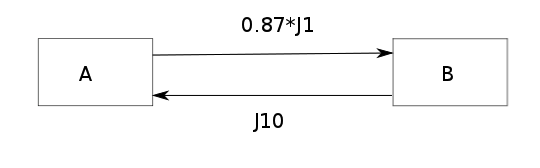
\includegraphics[width=5in] {pics/durationSwap}
\caption{$SW_{J1,J10}$ swap}
\label{fig:durationSwap}
\end{figure}

%I'm agreeing that in a year from now I'll pay $x$ J1s and receive a J10 (which will then be a J9 with price $100exp(-f(1,10))$ where $f(1,10)$ is the forward rate calculated as

%\[y_J(1,10) = \frac{10*y_J(0,10)-1*y_J(0,1)}{10-1} = \frac{10*0.015 - 0.01}{9} = 0.0156 \]

%(Remember that this forward rate exists by arbitrage) To make the swap have a zero net present value we solve

%\begin{eqnarray*}
%x*100*exp(-y_J(0,1)) = 100*exp(-y_J(1,10)*9)*exp(-y_J(0,1)) \\ 
%\Rightarrow x \approx 0.87
%\end{eqnarray*} 

We assume that the swaps are available in unlimited quantities. We'll call the swap $SW_{J1,J10}$ for short. Dealing with the swap directly makes things a lot more clear: it is  a bet on interest rates. Specifically it is a bet that in a year's time the yield of a J10 with 9 years left to maturity will be less than the forward rate 1.56\%. This is the rate for the J10 that makes V(1)=0. The payoff diagram is in figure \ref{fig:swap}. Notice that the payoff is slightly non-linear as a result of the non-linearity of the underlying bond.

\begin{figure}[ht]
\centering

\subfigure[As a function of price]{
   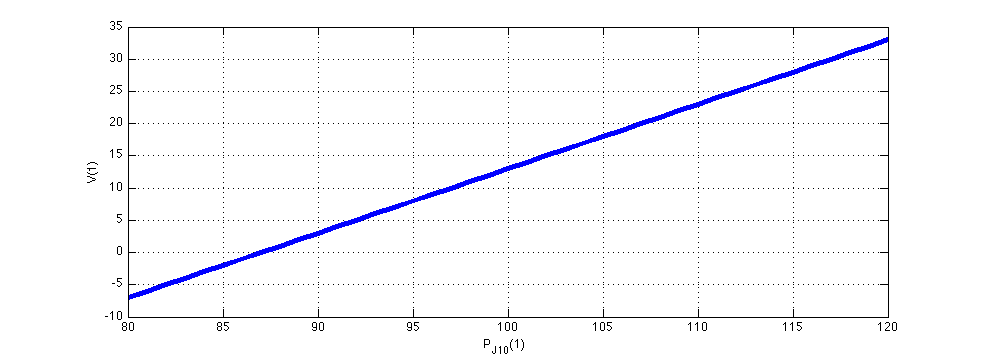
\includegraphics[width=3in] {pics/durationSwapP}
   \label{fig:durationSwapP}
 }

 \subfigure[As a function of future yield]{
   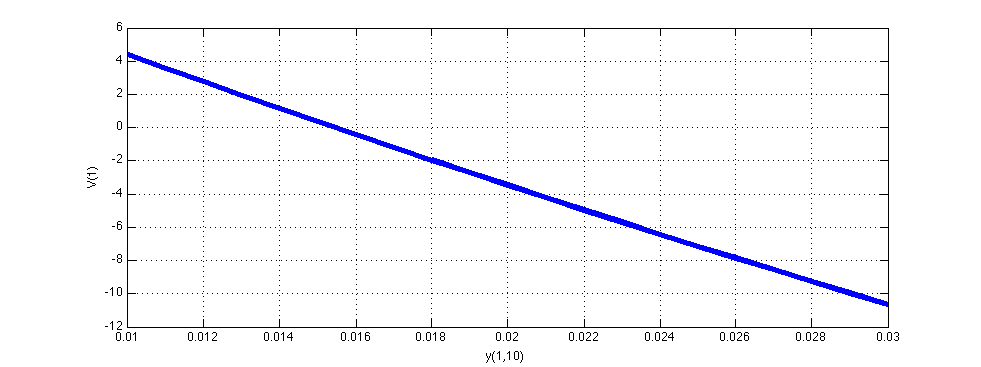
\includegraphics[width=3in] {pics/durationSwapR}
   \label{fig:durationSwapR}
 }
\caption{$V(1)$ for swap}
\label{fig:swap}
\end{figure}

\subsection{The credit objective}

We just used a swap to manufacture a pure bet on risk free interest rates. We can do a similar thing to manufacture a bet on whether Steve will repay his loan. Such a swap serves a useful purpose since the only reason anybody would lend to Steve rather than Jesus is the higher yield he pays on the bond. It's convenient to bet on Steve's creditworthiness directly.  Don't get too excited yet, but we're about to make a Credit Default Swap.

\textbf{A Jesus financed Steve portfolio}\\

We can buy an S1 by short selling 98.02/99.01 = 0.99 J1s. After a year we pay 100*0.99 = \$99 on our short Jesus and receive some amount (hopefully \$100) from Steve. But we might not get the whole \$100 from Steve. He's a shifty character, and there's a possibility he'll repay some lesser proportion $R$ of the \$100 when the bond comes to maturity. 

The current value of the portfolio is:

\[V(0) = -0.99*P_{J1}(0)+P_{S1}(0) = 0 \]

And after one year:

\[V(1) = -0.99*100 + P_{S1}(1)  = -99+ R*100 \]

The yield (in dollars) is

\[ \frac{\partial V}{\partial t}  = -y_{J1}*0.99*P_{J1}+y_{S1}P_{S1} = 0.9802 \]

So the current yield is around \$0.98 per year.

The portfolio has a dollar duration (DV01) of 

\[ \frac{\partial V}{\partial \bar{y}} =  -0.99*DV01_{J1}+1*DV01_{S1} = 0  \]
 
Which means that a one basis point increase in both Jesus and Steve's one year rate will have close to no effect (the sensitivity is zero, but the pricing function is convex so the effect isn't exactly zero). What matters in this transaction is the \textit{difference} between the  two rates, and ultimately the difference between the money you pay to cover the short Jesus and the amount you get back from Steve. Some people like to create a sensitivity measure called \textbf{spread duration} that gives the DV01 sensitivity of a portfolio to changes in the yield spread between the two bonds.  We can see better if we specify the yield on the S1 as the yield on the J1 plus a spread, then:

\begin{eqnarray*}
V(0) &= -0.99*P_{J1}(0) + P_{S1}(0)\\
 &= -0.99*100*\exp(-y_J(0,1))+100*\exp(-(y_J(0,1)+S)) 
 \end{eqnarray*}

Where $S$ is the spread (1\%). 

The spread duration is just the yield sensitivity on the S1:

\[ \frac{\partial V}{\partial S} = T *100*\exp(-(y_J(0,1)+S)) = 1*100*(\exp(-0.02*1)) = 0.0098 \]

So each 1bp increase in the spread costs the swap \$0.0098.

\textbf{A credit default swap representation}\\

This arrangement described is a swap. After one year the swap pays 0.99 J1s  and receives an S1. By assumption $P_{J1}(1) = 100$ and $P_{S1}(1) = 100*R$. This is a kind of \textbf{credit default swap} because the future value depends on the amount of the default. The swap is in figure \ref{fig:creditSwap}, the payoff profile after a year is in figure \ref{fig:CDSR}.

\begin{figure}[ht]
\centering
  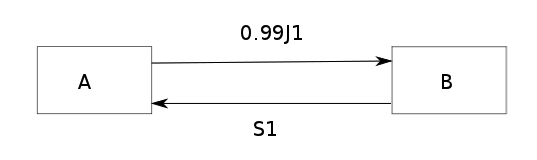
\includegraphics[width=5in] {pics/creditSwap}
\caption{$SW_{J1,S1}$ swap}
\label{fig:creditSwap}
\end{figure}

\begin{figure}[ht]
\centering
  \includegraphics[width=5in] {pics/CDSR}
\caption{$V(1)$ for CDS as a function of repayment rate}
\label{fig:CDSR}
\end{figure}

We'll call this swap $SW_{J1,S1}$. You can think of the 0.99 as the swap rate. It's a convenient way to bet Steve's credit worthiness without having to put up any cash up front.

This is a \textit{kind} of credit default swap but usually these are specified differently. Usually a CDS pays a certain amount now for protection against default later. The up front price is just the difference between the two bonds: S1-J1 = 99.02-98.01 = 1.01. It has to be because holding the swap \textit{and} an S01 gives the same payoff as a J01. 

The character of two remaining swaps $SW_{S1,J10}$ and $SW_{S1,S10}$ is left as an exercise.

\subsection{Summary}

\textbf{The duration objective}:\\
To trade the forward rate between $T_1$ and $T_2$ ($T_1<T_2$) for a risk free borrower $A$:
\begin{itemize}
\item Short sell $P_{AT_2}(0)/P_{AT_1}(0)$ of the $AT_1$s\\
\item Buy one of the $AT_2$s
\end{itemize}

At $t=0$ this portfolio has zero value. At $t=T_1$

\[V(T_1) = -\frac{P_{AT_2}(0)}{P_{AT_1}(0)}P_{AT_1}(T_1) + P_{AT_2}(T_1)   \]

The only uncertain variable is the $P_{AT_2}(t)$ price. This depends on the prevailing yield at $t=T1$. The breakeven for this trade is at the forward rate $f_A(T_1,T_2)$. The process is encapsulated in the \textbf{swap} $SW_{AT_1,AT_2}$

\textbf{The credit objective}:\\
To trade the credit of some risky borrower $B$ at a maturity $T$:

\begin{itemize}
\item Short sell $P_{BT}(0)/P_{AT}(0)$ of the $AT$s (the risk free bond)\\
\item Buy one of the $BT$s (the risky bond)
\end{itemize}

At $t=0$ the portfolio has zero value. At $t=T$

\[ V(T) = \frac{P_{BT}(0)}{P_{AT}(0)}P_{AT}(T) + P_{BT}(T) \]

The price of $AT$ is guaranteed since the bond is risk free, the price of $BT$ is linear in the recovery rate on the bond $R$. The process is encapsulated in a \textbf{credit default swap} $SW_{AT,BT}$.


\section{Trading}

A fixed income trader has two related tasks: 

\begin{enumerate}
\item Construct forecasts of future interest and repayment rates.\\
\item Construct a combination of trades to create a desired portfolio
\end{enumerate}

The first task is tricky.  A set of arbitrage free prices gives us almost no useful information. We can know the risk neutral expectations, -- the forward rates and forward spreads -- but those are the rates that give us zero profit. To forecast we have to bring some insight from outside. This might be some unexploited statistical regularity, or some superior understanding of the operation of a particular market.  These things are outside the scope of this chapter. Here we will focus on the second task. 

Swaps are a more direct way to bet on future interest rates and default rates than investing in bonds separately. It is almost always best to hold the minimum number of cash bonds in a portfolio. Most fixed income funds have the majority of their money in very short term securities with a collection of swaps (and other more exotic things) to transform the yield curve and credit exposure. It is common for a particular bond to trade thinly or not at all while a swap that creates the same exposure is highly liquid. 

In this section we'll demonstrate a few techniques for constructing trades.

\subsection{Hitting yield and DV01 targets}

The job of a fixed income trader is to construct a portfolio with some desirable characteristics. For example a client might want an unfunded portfolio to yield \$10 a year, with a spread duration of precisely \$0.05. Since portfolios sensitivities are linear in the instruments this is easy to do. 

If we just wanted to get to \$10 yield we could do it with both swaps from the previous section.  The $SW_{J1,J10}$ has a \$0.403 yield so we need $10/0.403 = 23.24$ times the exposure of the swap to get to \$10.  Increasing the exposure means increasing the notional value. If we increase the \textbf{notional value} by 23.24 times  from \$100 to \$2324 on the $J10$ leg of the swap. The $SW_{J1,S1}$ has  a yield of \$0.9802 so we need $10/0.9202 = 10.20$ times the exposure on the $S1$ leg -- a notional value of \$1020. 

\begin{tabular}{|c|ccccc|}
\hline
 & $J1$ face value & $J10$ face value & $S1$ face value & Yield & Spread duration\\
\hline
$SW_{J1,J10}$ & -87 & 100 & 0 & 0.403 & 0\\
$SW_{J1,S1}$ & -99 &  0 & 100 &  0.9802 & 0.0098\\
\hline
\end{tabular}

The spread duration of a \$100 notional value $S_{J1,S1}$ is 0.0098 so we'll need $0.05/0.0098 = 5.10$ times the exposure (\$510 notional value). This gives a yield of \$5 so we need to get the other \$5 of yield from 100*5/0.4303 = \$1162 notional value in the $SW_{J1,J10}$ swap.

One way to view these type of problems is as a set of linear constraints. Figure \ref{fig:yieldDV01} has the combinations of notional values required to hit the yield (blue line) and spread duration (red line) constraints. Each extra restriction is a line in this space. For simple problems this can be viewed graphically, more complicated problems can be solved with straightforward linear programming techniques (or if you're lucky just by solving a set  of linear equations). 

\begin{figure}[ht]
\centering
  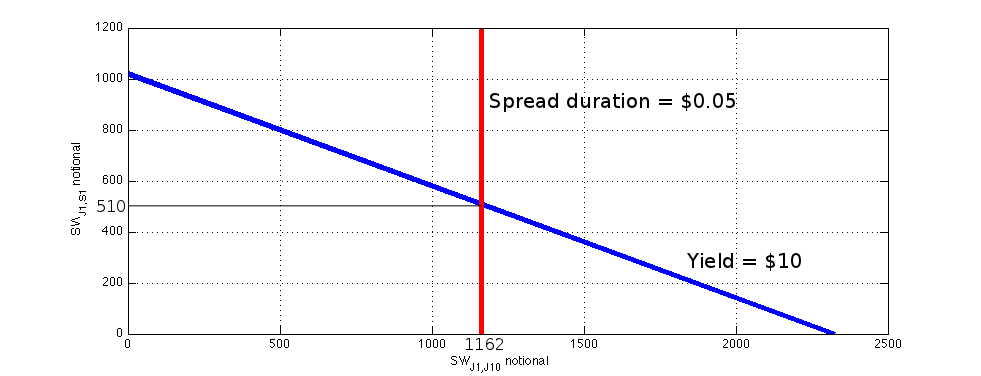
\includegraphics[width=5in] {pics/yieldDV01}
\caption{Notional swap value combinations to hit DV01 and yield targets}
\label{fig:yieldDV01}
\end{figure}

\subsection{Trading the curve}

We've constructed trades to have exposure to a particular forward rate. It's also possible to construct trades that have exposure to more than one forward rate. These combination trades allow traders to express more general views. For example it's possible to construct a trade to bet that the future yield curve will be \textbf{steeper or flatter} than the current forward curve suggests. It's also possible to construct a trade that the curve will be \textbf{more or less convex}.

We'll do this all with swaps. To give a bit more texture to the example we'll add a two more maturities for the Jesus bonds. The zero coupon yields and the nearby forward yield is in the table below.

\begin{center}
\begin{tabular}{|c|ccccc|}
\hline
Maturity & 1 & 2 & 3 & 5 & 10\\
Yield & 1\% & 1.056\% & 1.111\%& 1.22\% & 1.5\%\\
Forward &  & f(1,2) = 1.11\% & f(1,3) =1.167 & f(1,5) = 1.28\% & f(1,10) = 1.56\%\\
\hline
\end{tabular}
\end{center}

The swaps paying the one year bond  are $SW_{J1,J2}$, $SW_{J1,J3}$, $SW_{J1,J5}$, and $SW_{J1,J10}$. Each swap has final payoff that depends on one of the three forward rates. We'll calculate the DV01 in terms of these forward rates, and a reciprocal which is the notional value of the swap (on the receive side) that gives \$1 in DV01 to the forward rate. 


\begin{center}
\begin{tabular}{|c|c|c|c|}
\hline
Swap & Forward rate & DV01 to forward rate at $t=1$ & notional per \$1 of DV01\\
\hline
$SW_{J1,J2}$  & f(1,2) & $1*100*\exp(f(1,2)*1)/10000 = 0.0101$ & 100/0.0101 = 9889.5\\ 
$SW_{J1,J3}$  & f(1,3) & $2*100*\exp(f(1,3)*2)/10000 = 0.0205$ & 100/0.0205 = 4884.7\\ 
$SW_{J1,J5} $ & f(1,5) & $4*100*\exp(f(1,5)*4)/10000 = 0.0405$ & 100/0.0405 = 2468.3\\ 
$SW_{J1,J10}$  & f(1,10) & $9*100*\exp(f(1,10)*9)/10000 = 0.0914$ & 100/0.0914 = 1094\\ 
\hline
\end{tabular}
\end{center}

We'll also need the notional value of the underlying bonds and the dollar yields:

\begin{center}
\begin{tabular}{|c|ccc|}
\hline
Swap & $J1$ face value & Receive face value & Yield  \\
\hline
$SW_{J1,J2}$  & 97.91 & 100  & 0.5483  \\ 
$SW_{J1,J3}$  & 96.72  & 100  & 0.1064   \\ 
$SW_{J1,J5} $ & 95.08  & 100  & 0.207  \\ 
$SW_{J1,J10}$  & 86.07 &  100 &0.4304  \\ 
\hline
\end{tabular}
\end{center}

Now we're ready to trade the curve!

\subsubsection{Trading the level}

Say we believe that the forward curve will be uniformly higher across all maturities at $t=1$. Since the swaps have a negative exposure to the rate we'll need to sell swap (pay the long rate, receive the short rate). We can trade this with any of the three swaps in proportion to their DV01. To get the same exposure the $SW_{J1,J5}$ needs 2468.3/1094 = 2.25 times the exposure of the $SW_{J1,J10}$; or 9889.5/1094 = 9.04 times the exposure of the $SW_{J1,J2}$.

The picture is figure \ref{fig:level}.

\begin{figure}[ht]
\centering
  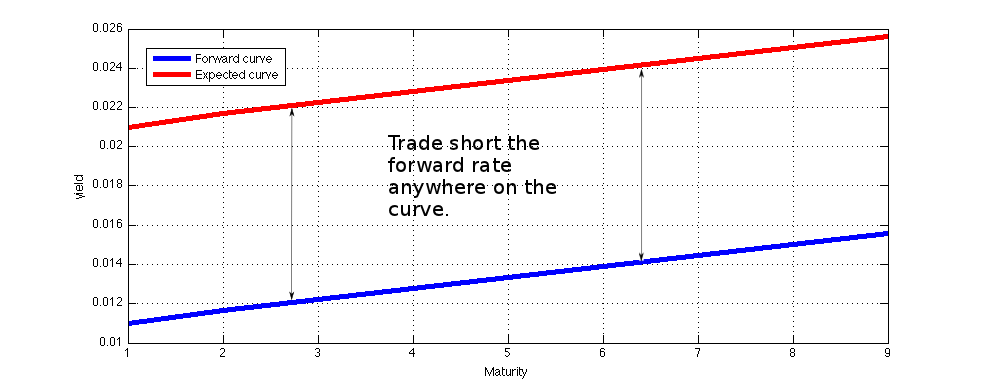
\includegraphics[width=5in] {pics/level}
\caption{Forward curve against expected future spot curve}
\label{fig:level}
\end{figure}

\subsubsection{Trading the slope: steepeners and flatteners}

Say we believe that the future yield curve will be steeper than the forward curve. We can trade this by buying the $SW_{J1,J2}$ and selling the $SW_{J1,J10}$ in proportion to their DV01s. To get \$1 of exposure each side we need \$9889.5 of notional from the $SW_{J1,J2}$ and \$1094 of notional from the $SW_{J1,J10}$. The trade will make more money if the future curve is steeper than the forward curve. This trade, and trades with the same effect, are called \textbf{steepeners}.

If we believe the future curve will be flatter we can do the opposite trade. Then it is called a \textbf{flattener}.

Notice that the level of the curve doesn't affect the trade (except a little through convexity). The curve could end up entirely above or below the current forward curve and the trade would still have the same (approximate) effect. All that matters is the slope of the curve between the 4 and 9 year maturities.  Note also that the trade is \textbf{duration neutral}. The picture is figure \ref{fig:slopes}.

\begin{figure}[ht]
\centering

\subfigure[Steepener]{
   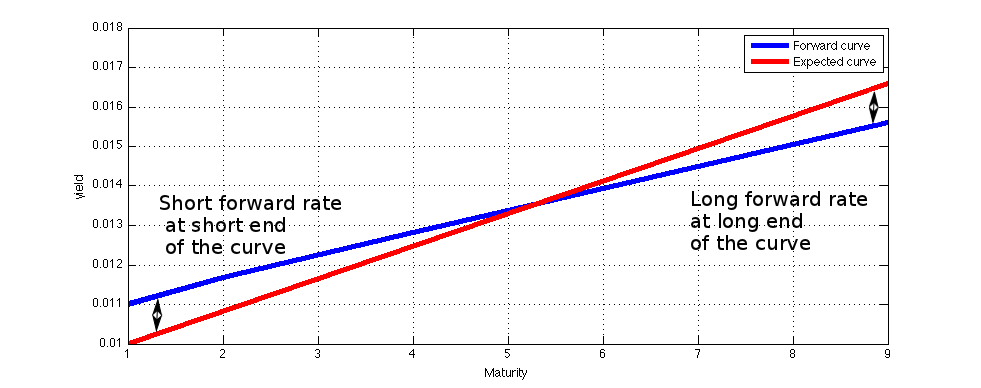
\includegraphics[width=3in] {pics/steepener}
   \label{fig:steepener}
 }

 \subfigure[Flattener]{
   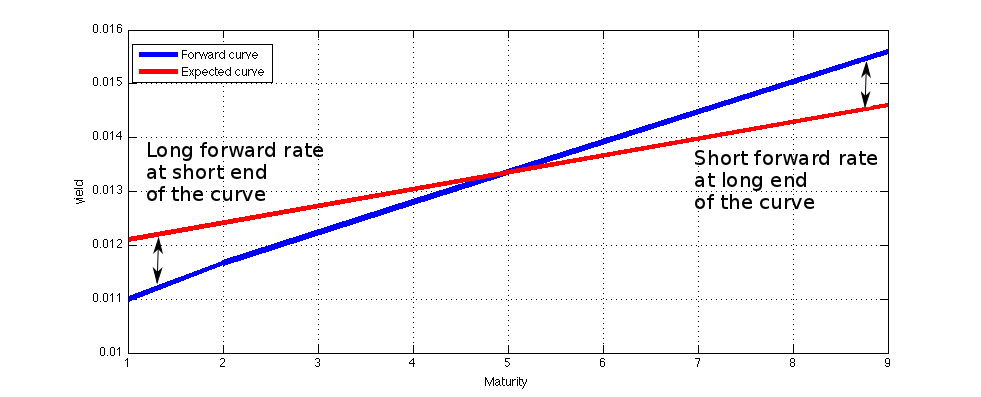
\includegraphics[width=3in] {pics/flattener}
   \label{fig:flattener}
 }
\caption{Curve slope trades}
\label{fig:slopes}
\end{figure}

\subsubsection{Trading convexity}

Supposing instead we thought the future curve would be more convex than the forward curve. In our example the forward curve is linear so any convexity will do. A convexity trade requires three points on the curve: one long rate, one short rate, and one middle rate. Our belief in future convexity of the curve means we think the curve will bend inwards, with the long and short rate decreasing by more than the middle rate (see picture). For this we buy DV01 adjusted amounts of $SW_{J1,J2}$ and $SW_{J1,J10}$ and sell \textit{twice} as much DV01 adjusted $SW_{J1,J5}$ to make the trade duration neutral.

This trade is commonly called a \textbf{butterfly} (the long and short rate trades are the `wings' of the insect, the middle rate trade is the body). We could also do the trade in reverse if we thought the future curve would be less convex than the forward curve. The picture is figure \ref{fig:butterfly}.

\begin{figure}[ht]
\centering
  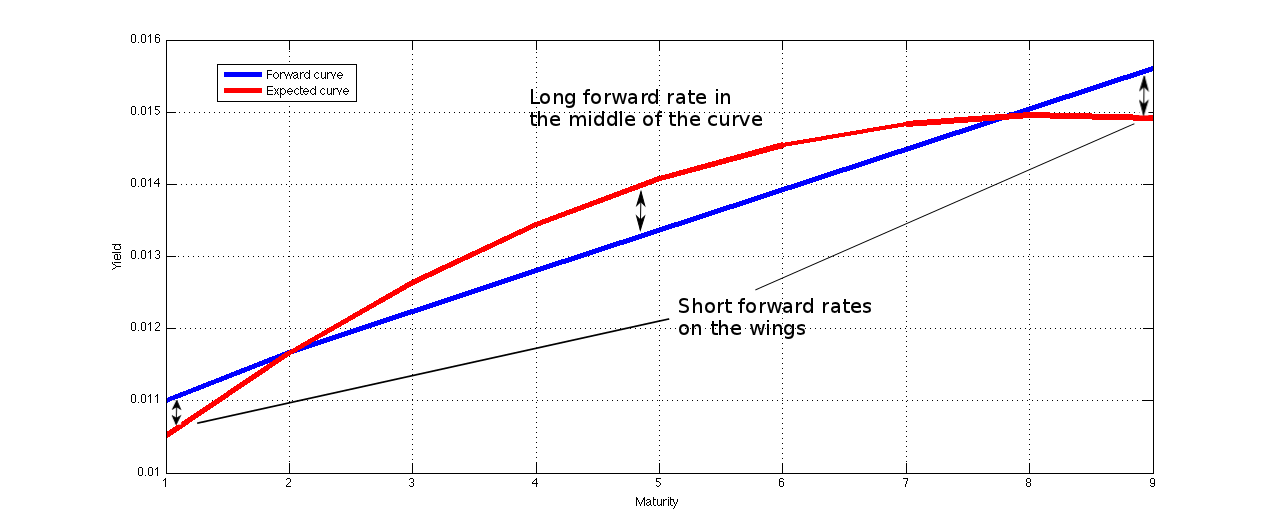
\includegraphics[width=5in] {pics/butterfly}
\caption{Butterfly}
\label{fig:butterfly}
\end{figure}

\subsection{Trading credit}

Trading credit is similar to trading rates. A credit trade is a bet on the future market expectation of default. If a company actually defaults there is usually still some uncertainty over how much a sale of assets will return bondholders.  For each borrower there is a curve giving the spread against a less risky bond (usually the government curve). This curve can be traded in the same way as rates: with steepeners and flatteners and butterflies and such.

To trade the possibility of default directly we can trade either $SW_{J1,S1}$ or $SW_{J10,S10}$. Both give a direct exposure to the default rate at $t=1$ and $t=10$. Trading $SW_{J1,S10}$ gives an exposure to the nine year \textbf{forward rate} on the S10 one year forward.

Individual CDSs often have a large \textbf{bid offer spread} because the underlying bonds are difficult to buy and sell. This leads many to trade \textbf{credit default swap indices} based on the \textbf{credit spread} of a number of different entities. There are different indices for different credit classes, as well as for geographical and industry groupings. There are a number of other widely traded credit derivatives: \textbf{Collateralised Debt Obligations} (CDOs) are instruments that take some portion of the credit exposure from a bond, or from a collection of bonds. There are also options on bonds, rates (caps/floors), and swaps (swaptions), and an endless rainbow of exotic derivatives. 

There is a lot more to say about  credit instruments and trading, but we'll leave the discussion to the discussion on credit.

\subsection{Hedging interest rate risk}

Fixed income trading isn't all punting on rates and spreads. There is the occasional legitimate hedger. Businesses wish to remove interest rate risk, either from existing floating rate loans, or for future loans they intend to make or receive. This hedging can be done in (at least) two ways: either with swaps for each uncertain payment, or a single swap on all uncertain payments.

In both cases the swap is priced by finding  a fixed rate that makes the fixed and floating legs of the swap equal discounted values. Uncertain future rates are evaluated at the forward values (e.g. $y(2,3)$ is given the value $f(2,3)$).

%as a trade on a single future rate, or on a series of rates. If the business already has a floating rate loan, it's a simple matter to create a fixed-for-floating swap to remove the uncertainty associated with the future interest rate rises. Each uncertain future rate has a market determined forward rate, a \textbf{fixed for floating swap} replaces regular uncertain (floating) payments by regular fixed payments. The fixed rate is the rate that makes the present value of all floating payments evaluated at the appropriate forward rate equal to the present value of the fixed payments. 

\subsubsection*{Example: Hedging with multiple swaps}
Say that you are short a bond with a \$100 face value with a \textbf{floating coupon} equal to the Jesus rate (risk free) + 2\%. The bond maturity is 2 years, and coupons are paid annually. You are exposed to the risk that the Jesus rate will increase. 

For the first payment the swap rate is the forward value of the payments, which is the forward rate plus 2\%:

\begin{center}
\begin{tabular}{|ccc|}
\hline
Time & floating payment & fixed payment\\
\hline
1 & $100*(y_J(1,2)+0.02)$ &  $100*F_1$\\
\hline
\end{tabular}
\end{center}

The swap rate is $F_1 = f(1,2)+0.02 =$ 3.11\%.

Similarly for the second payment:

\begin{center}
\begin{tabular}{|ccc|}
\hline
Time & floating payment & fixed payment\\
\hline
2 & $100*(y_J(2,3)+0.02) + 100$ & $100*F_2 + 100$\\
\hline
\end{tabular}
\end{center}

The swap rate is $F_2 = f(2,3) + 0.02 =$ 3.22\% 


%To hedge this risk you can enter into two \textbf{forward rate agreements}, one for each coupon. These agreements specify that you can borrow at a future point in time for a fixed rate. These will each be priced at the forward rates $y(1,2) = 1.11\% $ and $y(2,3) = 1.22\%$. With these FRA's in your top drawer you are guaranteed to pay in net 1.11+2 = 3.11\% for the first coupon and 1.22+2 = 3.22\% for the second coupon. WRONG BECAUSE FRA IS LINEAR 

\subsubsection*{Example: Hedging with a single swap}
We can also hedge out the risk with a swap which pays a fixed coupon and receives the floating rate. The swap payments look like this (we'll call the fixed rate $F$):

\begin{center}
\begin{tabular}{|ccc|}
\hline
Time & floating payment & fixed payment\\
\hline
0 &  & \\
1 & $100*(y_J(1,2)+0.02)$ &  $100*F$\\
2 & $100*(y_J(2,3)+0.02) + 100$ & $100*F + 100$\\
\hline
\end{tabular}
\end{center}

To get the swap rate we make the discounted values of these payments equal, with the uncertain future rates evaluated at the forward rates.

\begin{eqnarray*}
V(0) = \exp(-y(0,1)*1)*100*(f(1,2)+0.02) + \exp(-y(0,2)*2)*(100*(f(2,3)+0.02) +100) \\
- (\exp(-y(0,1)*1)*100*F + \exp(-y(0,2)*2)*(100*F+100))  = 0
\end{eqnarray*}

Which gives $F=3.1647\%$. By entering into the swap you remove the interest rate risk. You still pay the floating rate on the bond but the swap pays the difference between the floating coupon and the fixed swap rate.


\subsection{Summary}

Trading is mostly about constructing portfolios to do certain things: to hit sensitivity targets and/or to have an exposure to the forward curve. Hitting sensitivity targets is easy since bond and swap portfolios are linear in sensitivities. Constructing exposures to the forward curve is easy with swaps since swaps can be constructed to have a breakeven at any desired forward rate.

To get exposure to the a risk free forward rate $f_A(T_1,T_2)$ trade the swap $SW_{AT_1,AT_2}$ since this has

\[V(0) = \frac{-P_{AT_2}(0)}{P_{AT_1}(0)}P_{AT_1}(0) +  P_{AT_2}(0) = 0  \]

and

\begin{eqnarray*}
V(T_1) =& \frac{-P_{AT_2}(0)}{P_{AT_1}(0)}P_{AT_1}(T_1)+  P_{AT_2}(T_1)  \\
=& \exp(-y_A(0,T_2)T_2 + y_A(0,T_1)T_1)FV + \exp(-y_A(T_1,T_2)(T_2-T_1))
\end{eqnarray*}

Where $FV$ is the common face value for the bonds. The only uncertain value in the equation is the future rate $y_A(T_1,T_2)$. The swap breaks even at $T_1$ when 

\[y_A(T_1,T_2) = f_A(T_1,T2) = \frac{y_A(0,T_2)T_2 - y_A(0,T_1)T_1}{T_2-T_1}\]

If the bond is not risk free a the possibility of default can be removed with a CDS on the $AT_1$ bond.


\textbf{Hitting sensitivity targets}:\\
The dollar yield and sensitivity of a portfolio is the sum of the yields or sensitivities of its components. Increasing the position sizes (notional value of swaps) increases the sensitivity linearly. Combination sensitivity targets can be hit by solving the associated linear programming problem.

\textbf{Curve trades}:\\

\textit{Level}:\\
Trade any swap on the curve in proportion to its DV01 to the target forward rate.

\textit{Steepener}:\\ 
Generate a negative exposure to the forward rate at the short end of the curve and a positive exposure to the forward rate at the long end of the curve. Adjust both positions to have equal DV01 to the forwards.

\textit{Flattener}:\\
Opposite to a steepener.

\textit{Convexity:}\\
Generate a positive exposure to the forward rate in the middle of the curve and negative exposure to forward rates at the long and short end of the curve (the wings). Adjust positions to have twice the DV01 to the forward in the middle as on either of the wings.

\textbf{Credit trades}:\\
For pure default exposure swap risk free for risky bond at target maturity. 

\textbf{Interest rate hedging}:\\

\textit{Hedge each payment}:\\
Offset each payment with a different swap. 

\textit{Hedge all payments}:\\
Offset all payments with a single swap.


\section{Popular trading strategies}

The optimal trading strategy at any point in the future will depend on your view of the difference between the forward rates and the rates or spreads you expect to prevail in the future. This requires a forecast and forecasts are tricky. Fixed income traders are lazy by nature and don't like doing tricky things so they take the current yield curve as a predictor of the future yield curve. This gives rise to two of the most popular fixed income strategies: \textbf{carry} and \textbf{rolldown}.

In figure \ref{fig:genericCurve} the expected future curve is equal to the current zero curve (blue line). Differences between the current forward curve (red line) and the expected future curve can be traded easily with swaps or forwards as we did in the last section. 

\begin{figure}[ht]
\centering
  \includegraphics[width=5in] {pics/genericCurve}
\caption{Spot curve = expected future spot curve vs. forward curve}
\label{fig:genericCurve}
\end{figure}

\subsection{Carry trades}
The idea of a carry trade is to borrow money cheaply and lend it expensively. Since it's a lot of trouble to \textit{actually} borrow and lend money this is usually done with swaps or futures which give cashflows \textit{as if} you had done all the tiresome lending and borrowing. A trade with \textbf{positive carry} has the characteristic that it has a positive yield ($\partial V/\partial t$) when it is fully financed (zero cost up front). This is an attractive characteristic: you pay nothing and you start getting paid up front. These trades are not riskless; just because a trade has a positive yield now doesn't mean it will have a positive yield later, or that changes in rates and spreads will not cause it to lose money in the future. But still it's a nice characteristic, and historically many carry trades have been profitable for investors so they remain popular. A famous hedge fund manager called John Devaney bought a large and expensive yacht and painted the name `positive carry' on the side: no prizes for guessing how he got the money to buy it.

\textbf{Across curve carry:}\\

Rate curves usually slope up or down. A cross curve carry trade borrows money on a low rate part of the curve and lends on a high rate part of the curve. The yield of the carry will be proportional to the difference between the low rate and the high rate. For example if the 1 year rate is 1\% and the 10 year rate is 1.5\% we can enter a swap to pay the 1 year rate and receive the 10 year rate. We saw before the dollar yield for a 1x10 year Jesus swap is:

\[\frac{\partial V}{\partial t} = -y_{J1}*0.87*P_{J1}+y_{J10}P_{J10} = 0.4303  \]

There's our positive carry. The value after one year will be

\[V(1) = -0.87*100+100*\exp(-y_J(1,10)*9) \]

The breakeven $y(1,10) $ yield is 0.0156 (the forward yield). If the yield curve is linear the current 9 year yield is 0.0145. By trading the swap we're exploiting the difference between the current 9 year rate and the 9 year rate one year forward (see figure \ref{fig:carry}). If the yield curve maintains its shape we make money. Even if it moves against us a little we still make money.

\begin{figure}[ht]
\centering
  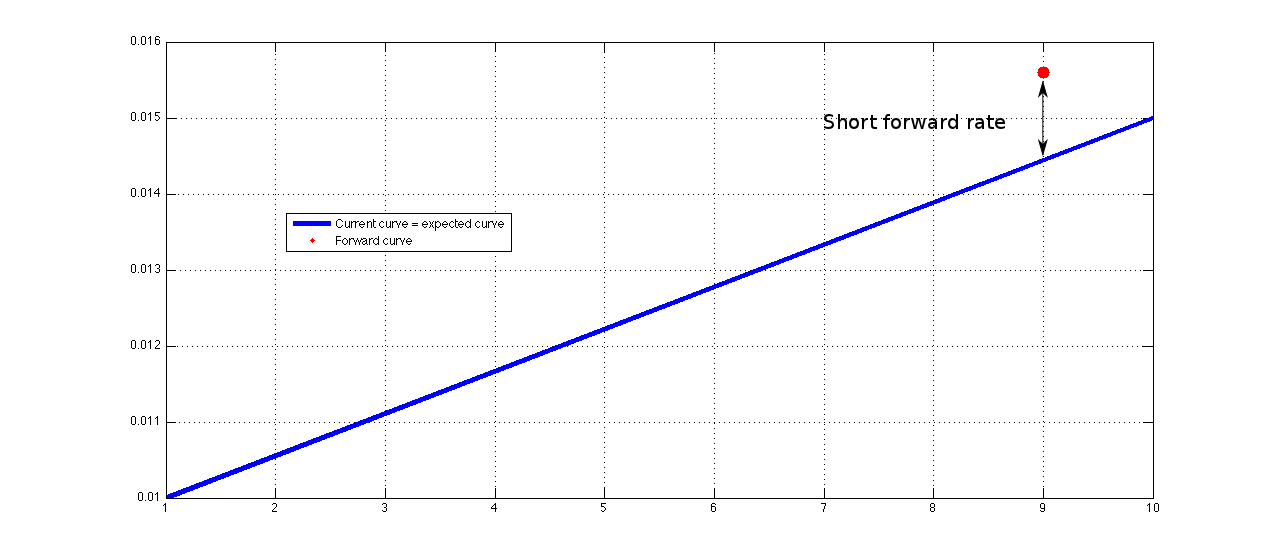
\includegraphics[width=5in] {pics/carry}
\caption{Carry trade when forward is different to current spot rate}
\label{fig:carry}
\end{figure}

We could get a very similar exposure by buying a properly priced bond future on the 10 year bond expiring in a year, or by buying a future on the the 9 year rate one year forward. All of these trades have the \textit{effect} of borrowing money at the low rate and lending it at the high rate.


\subsubsection*{Between curve carry:}

Rates differ across curves but also among curves.  A swap which pays a low rate and receives a high rate at the same maturity is also a carry trade. The $SW_{J1,S1}$ swap is an example. The swap pays the low Jesus rate and receives the high (and risky) Steve rate.

The swap has positive carry as a compensation for assuming the riskiness of the S1:

\[\frac{\partial V}{\partial t} = -y_{J1}*0.99*P_{J1}+y_{S1}P_{S1}= 0.9802 \]

Any other swap between curves with different yields can also be constructed with positive carry. The trick is to try to get the best carry for the least risk measured in spread duration, convexity, or whatever else you care about.


\subsubsection*{Cross currency carry:}

Rates differ between maturities and credit classes and also between countries. Riskless government bonds denominated in two currencies, will trade at different rates. Borrowing the cheap rate and lending the expensive rate is a carry trade.

The magic of arbitrage makes it unnecessary to actually borrow money in one country and lend it in another. The mechanics are bundled up into swaps and forwards. But the outcome is \textit{as if} you had borrowed and lent money. These can be used to convert loans in one currency to another or purely to extract the positive carry. We'll cover currency swap pricing in the next section so we won't go into it here but the basic idea is this: \textbf{if the low rate currency doesn't appreciate more than the interest rate difference the carry trade makes money}. 

\subsection{Rolldown trades}

Most yield curves are curvey, and some parts of the curve are curvier than others. Steep parts of the curve present an opportunity to a certain type of trader. If the curve retains its shape, the yield on a bond yield will \textbf{roll down} the curve, increasing the price of bond. The steeper the curve, the more pronounced the effect. Many fixed income strategies take advantage of this by positioning swaps and forwards on steep parts of the curve. We'll see in the example that this effect can be quite large, sometimes much larger than the pure carry, so it pays to be aware of rolldown even if you aren't trading it directly.

\begin{figure}[ht]
\centering
  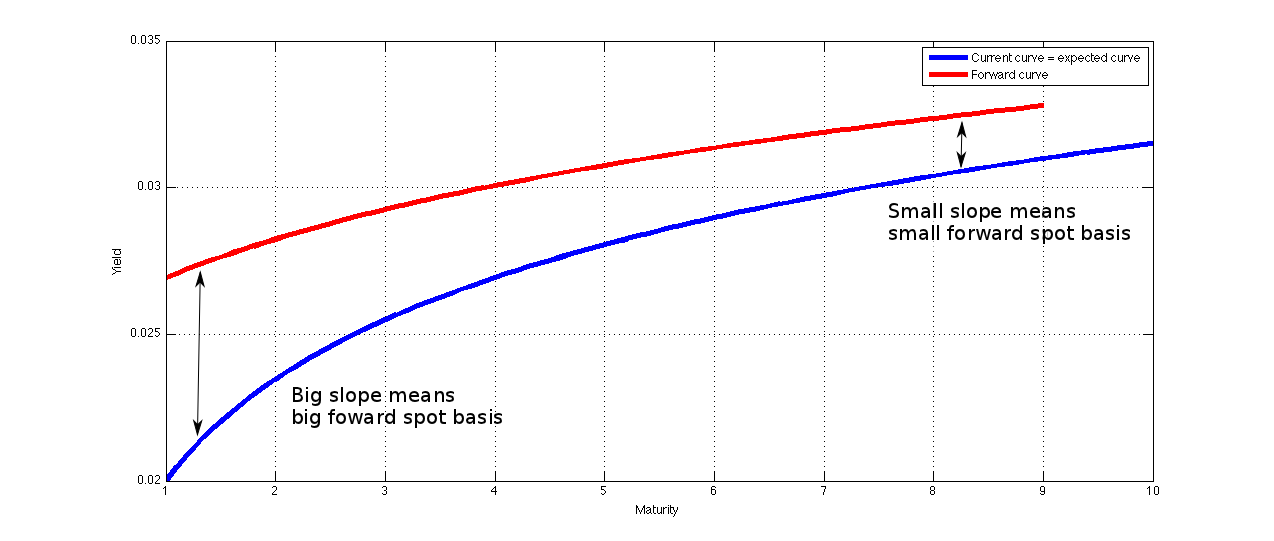
\includegraphics[width=5in] {pics/rolldown}
\caption{Rolldown trade on steep part of yield curve}
\label{fig:rolldown}
\end{figure}

%Example: y(T)  = @(T)(0.5*log(T)+2)/100;
%f = @(T2) (y(T2)*T2-y(1)*1)/(T2-T1)
%draw pic

The steeper the forward curve, the greater the difference between the forward rate and the spot rate, and so the greater the profit to the trade. Figure \ref{fig:rolldown} illustrates the effect on a convex yield curve: as the curve gets steeper the difference between forward and spot increases. 



One way to look at this is to decompose the value of a security into the yield and the rolldown. If we assume a constant slope $y(T)$ then the total yield is given the total derivative:

\[\frac{d V}{d t} = \underbrace{\frac{\partial V}{\partial y}\frac{\partial y}{\partial t}}_{\mbox{rolldown}} + \underbrace{\frac{\partial V}{\partial t}}_{\mbox{carry}}\ \]

It's similar with a swap whose value depends on a spread $S$ (which is a function of $y(T)$), then:

\[\frac{d V}{d t} = \underbrace{\frac{\partial V}{\partial S}\frac{\partial S}{\partial t}}_{\mbox{rolldown}} + \underbrace{\frac{\partial V}{\partial t}}_{\mbox{carry}}\ \]


\textbf{Example of a rolldown trade:}\\

We'll make a yield curve that is steep at the start and flattens out at longer maturities.\footnote{This one is $y(T) = (0.5*\ln(T)+2)/100$. In the real world yield curves don't have parametric forms but this makes the calculations easier.}  Table \ref{tab:rolldownTable} has the details. We proxy the slope of the spread curve $\frac{\partial S}{\partial t}$ by the slope of the chord connecting each adjacent spread. 

\[\mbox{Slope between $T_1$ and $T_2$} = \frac{\partial S}{\partial t} \approx \frac{y(0,T_2)-y(0,T_1)}{T_2-T_1} \]

This is an approximation but it's fine for our purposes.

\begin{center}
\begin{table}
\begin{tabular}{|c|cccccc|}
\hline
Maturity (years) & 1 & 2 & 5 & 6 & 10 & 11\\
Yield & 2\% & 2.34\% & 2.8\% & 2.90\%  & 3.15\% & 3.2\%\\  
1 year forward & & 2.69\% & 3.01\% & 3.08\% & 3.28\% & 3.32\% \\
spread to 1 year ($S$) & 0 & 0.34\% & 0.80\% & 0.90\% & 1.15\% & 1.2\%\\ 
$\frac{\partial S}{\partial t}$ & & -0.0034 & -0.0015 & -0.0009 & -0.0006 & -0.0005\\
\hline
\end{tabular}
\caption{Yields, forwards, spreads, and slopes}
\label{tab:rolldownTable}
\end{table}
\end{center}
%working in google docs 'working'


We know that we want to trade on the steep part of the curve, but we don't know exactly why yet. Everything becomes clear if we construct three swaps: $SW_{1,2}$, $SW_{1,6}$, and $SW_{1,11}$. (do this in the usual way, paying 1 year, receiving the longer maturity bond). The total yield is decomposed in table \ref{tab:decomposeSwap}:

\begin{center}
\begin{table}
\begin{tabular}{|c|cccccc|}
\hline
 & $\frac{\partial V}{\partial S}$ &$\frac{\partial S}{\partial t}$ & $\frac{\partial V}{\partial t}$ & $\frac{\partial V}{\partial S}\frac{\partial S}{\partial t}$ & $\frac{d V}{d t}$ & carry/rolldown\\
 \hline
$SW_{1,2}$ & -190.8 & -0.0034 & 0.331 & 0.661 & 0.992 & 0.5\\
$SW_{1,6}$ & -504.3 & -0.0009 & 0.753 & 0.460 & 1.213 & 1.64\\
$SW_{1,11}$ & -773.7&-0.0005 & 0.843 & 0.369 & 1.212 & 2.29\\
\hline
\end{tabular}
\caption{Decomposing swaps into carry and rolldown}
\label{tab:decomposeSwap}
\end{table}
\end{center}

Even though the $SW_{1,11}$ swap has a higher carry it has a lower expected total yield than the $SW_{1,6}$. Adjusted for spread duration ($\frac{\partial V}{\partial S}$) the $SW_{1,2}$ is clearly superior: it give a yield of around the same as the others with around a third the risk. The reason is that the effect of the additional carry gained from the higher yield of the 11 year bond is outmuscled by the rapidly declining yield of at the 1-2 year end of the curve. This is clear in the figure which shows the steep short end has the greatest difference between spot and forward rates. 

These kind of trades are wildly popular in fixed income funds, though often traders give more grand explanations. They are fairly persistently profitable, though still risky. A variant is to trade pairs with long positions on the steeper end of the curve and short positions on the flatter end. Another is to trade pairs across countries: long the steep curves and short the flat/inverted curves. The idea is to get the benefits of the rolldown while insulating the trade against global movements in yields. The exact implementation will depend as usual on risk preferences, liquidity, and such.

\subsection{Summary}

Carry trades borrow cheap money and lend expensive money. This can be done across a single yield curve or across different yield curves. Rolldown trades exploit an expectation that the curve will retain its shape by shorting the forward rate when the slope is large.


\textbf{Carry trades}:\\

\textit{Between curve carry}:\\

Enter a swap paying a low yield and receiving a high yield at different maturities.

\textit{Across curve carry}:\\

Enter a swap paying a low yield and receiving a high yield at the same maturity for two different borrowers.

\textit{Cross currency carry}:

Enter a swap to pay a low yield currency and receive a high yield currency at the same maturity.

\textbf{Rolldown trades}:

Enter a swap that is short the forward rate at a maturity where the curve is steep or long the forward rate when the curve is steeply negative.

\section{Currency and inflation}

We'll look at two swaps: a \textbf{cross currency swap} and an \textbf{inflation swap}. To construct these swaps we follow the same three step process we did for rates and credit:

\begin{enumerate}
\item Set a target exposure for the swap (e.g. the currency exchange rate)\\
\item Find two instruments which differ only in the target exposure (e.g. a bond from country A and a bond from country B at the same maturity)\\
\item Create a self financing (zero cost) portfolio by buying and short selling (paying and receiving) the two instruments\\
\end{enumerate}

And wallah! You've got your target swap. 

\subsection{A currency swap}

There are two countries: Australia and Barbados. Both issue 1 year bonds which are for the sake of the story are risk free. Australia issues in Australian dollars prefixed $\$A$, Barbados issues in Barbadian dollars prefixed $\$B$. Both bonds have a face value of 100 in the local currency. The exchange rate between the two countries is $X_{\$A,\$B}$, the number of Australian dollar for each Barbadian dollar. 

\begin{center}
\begin{tabular}{|c|ccc|}
\hline
 & Yield & Price & Exchange rate\\
 Australia 1 year bonds (A1) & 1\% & 99.01 & $X_{\$A,\$B}(0) = 0.5$\\
 Barbados 1 year bonds (B1) & 2\% &  98.01 &$X_{\$B,\$A}(0) = 2$\\
\hline
\end{tabular}
\end{center}
 
 The cost of a Barbados bond in Australian dollars is $98.01*0.5 = 49.01$. To purchase one Barbadian bond costs 49.01/99.01 = 0.495 Australian bonds. The self financing portfolio is short 0.495 Australian bonds and long 1 Barbados bond.
 
 \[V(0) = -0.495*P_{A1}(0) + P_{B1}(0)X_{\$A,\$B}(0) = 0 \]
 
 After one year both bonds mature and we pay \$A49.5 and receive \$B100. Exchange the \$B100 back at the prevailing exchange rate in 1 year and the total payoff is
 
 \[V(1) = -0.495*P_{A1}(1)+100*X_{\$A,\$B}(1) \]
 
The breakeven for this trade is when $X_{\$A,\$B}(1) = 0.495$ (see figure \ref{fig:currency}). If the exchange rate is greater the swap makes money. This means we can afford for the Australian dollar to drop 1\% against the current exchange rate and still make money. 
 
 The carry in Australian dollars is positive:
 
 \[\frac{\partial V}{\partial t} = -y_{A1}*0.495*P_{A1} + y_{B1}*P_{B1}*X_{A\$,B\$} (0)= 0.49 \]

The only uncertainty is the currency, so the currency swap is a pure linear exposure to the future exchange rate.

\begin{figure}[ht]
\centering
  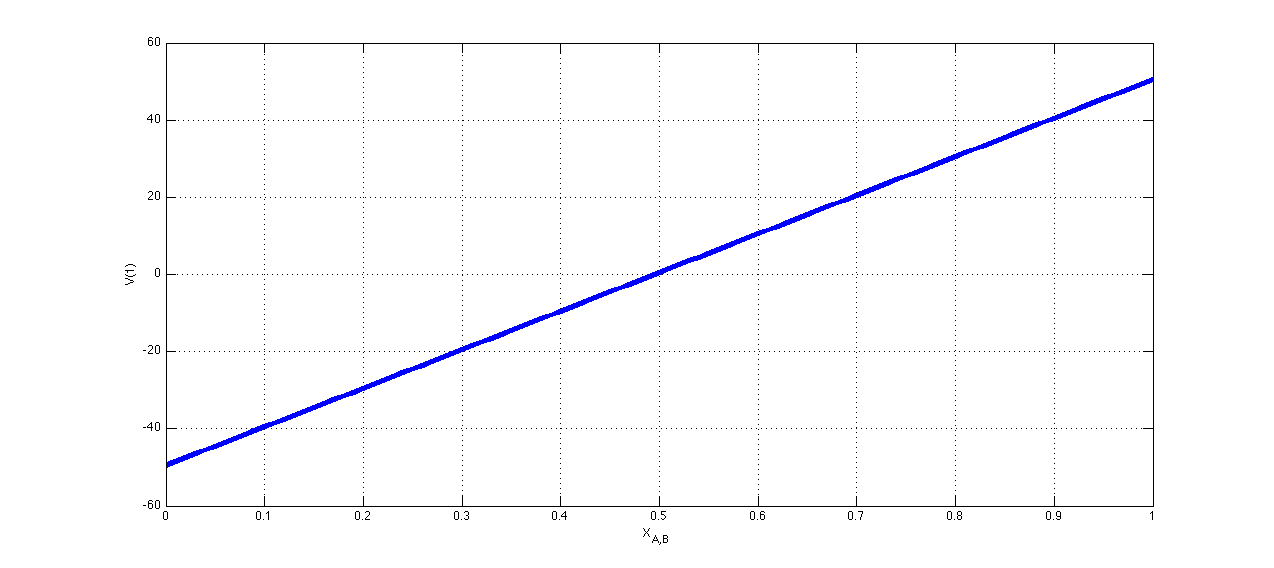
\includegraphics[width=5in] {pics/currency}
\caption{Currency swap payoff}
\label{fig:currency}
\end{figure}
 
\subsection{An inflation swap}

The problem with borrowing money from governments is that they have it in their power to create money to pay off their debts.  Printing money will lead to inflation, which means the money in the future is less valuable. Bond yields will account for this: borrowers will demand a higher yield to compensate for the loss of value in the currency at maturity. In many instances the quantum of this \textbf{inflation premium} is unobservable; it is mixed in with the real yield. However sometimes governments issue \textbf{inflation linked bonds} with a face value (and/or coupon) linked to a measure of inflation. These bonds can be stripped of the inflation component which prices separately as an \textbf{inflation swap}.

Inflation linked bonds come in a few flavours but here we'll take a zero coupon bond that repays $100*(1+I)$ at maturity where $I$ is the increase in some inflation measure (usually the Consumer Price Index).  A inflation linked bond and a normal bond trade at \$99.01 and \$99.5. 

\begin{center}
\begin{tabular}{|c|ccc|}
\hline
 & Yield & Price  & Face value \\
 \hline
1 year bonds (A1) & 1\% & 99.01 & 100 \\
1 year inflation linkers (I1) & ?\% &  99.5 & $100(1+I)$\\
\hline
\end{tabular}
\end{center}

We don't know what the yield of the linker is because we don't know what $I$ will be. We can however determine the market price of inflation by constructing a swap short 99.5/99.01 = 1.005 normal bonds and long one linker. 

The swap is self financing:

\[ V(0) = -1.005*P_{A1}(0) + P_{I1}(0) = 0\]

At expiry we have

\[ V(1) =  -1.005*100 + 100*(1+I)\]

This is a fixed for floating swap: the fixed rate is 1.005 and the floating rate is $(1+I)$. The swap is  a linear exposure to future inflation which breaks even when $I=0.005$. The market expects inflation to run at 0.5\% for the year. 

\begin{figure}[ht]
\centering
  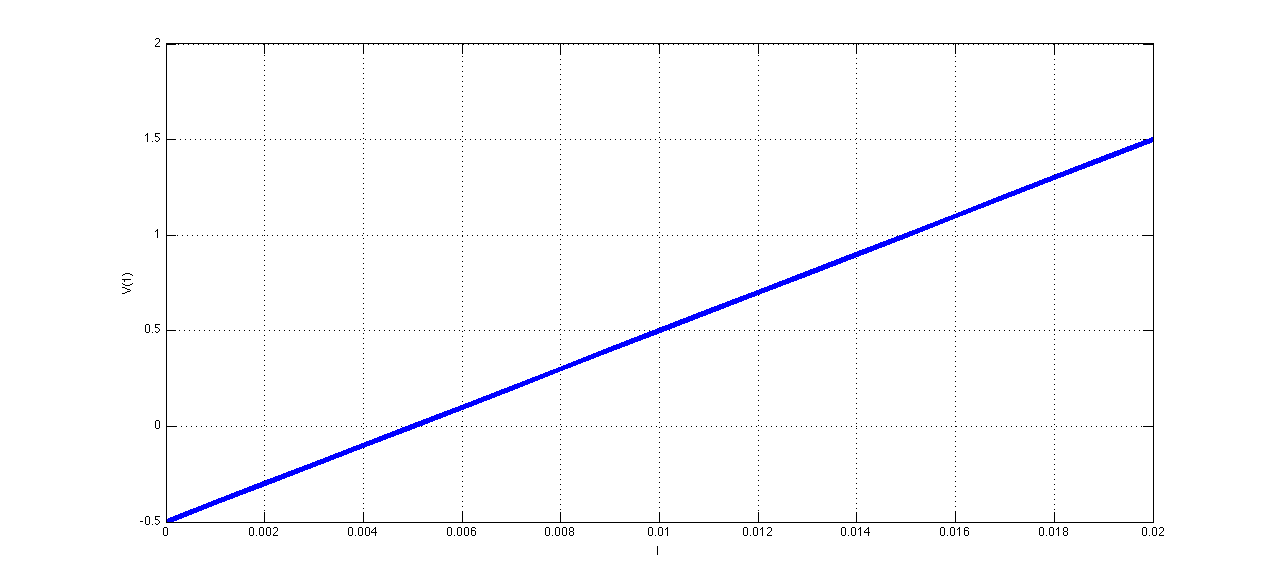
\includegraphics[width=5in] {pics/inflation}
\label{fig:inflation}
\caption{Inflation swap payoff}
\end{figure}

\subsection{Summary}

A currency swap pays and receives in two different currencies, an inflation swap pays a fixed face value and receives a face value dependent on the inflation rate.

\textbf{A currency swap}\\
Enter a fully financed swap paying a bond in currency $A$ and receiving a bond in currency $B$ at the same maturity. This gives an exposure to the forward exchange rate.

With arbitrary yields and maturity $T$ the swap has the following payoff in \$A:

\begin{eqnarray*}
V(T) = -\frac{P_{BT}(0)}{P_{AT}(0)}*P_{AT}(T)+ P_{BT}(T)*X_{\$A,\$B}(T) \\
 =  FV_A\exp((-y_{BT}+y_{AT})*T)+ FV_B*X_{\$A,\$B}(T)  
 \end{eqnarray*}

where $X$ is the exchange rate and $FV$ is the face value of the bonds. The only uncertain value is the future currency rate $X_{\$A,\$B}(T)$.

\textbf{An inflation swap}

Enter a swap to pay a normal bond $AT$ and receive an inflation linked bond $IT$ with the same maturity. The resulting exposure is the inflation linked portion of the linker. 

\begin{eqnarray*}
V(T) = \frac{P_{IT}(0)}{P_{AT}(0)}*P_{AT}(T)+ P_{IT}(T) \\
 =  FV\exp((-y_{IT}+y_{AT})*T)*P_{AT}(T)+ FV(1+I)  
 \end{eqnarray*}

The only uncertain value is the inflation rate $I$.


\section{Questions}

\textbf{Question 1:}\\
Consider the swap $SW_{J1,S10}$ from the credit and duration section. 

\begin{itemize}
\item[(a)] Give the equations for $V(0)$, $V(1)$
\item[(b)] Calculate the dollar yield and spread duration.
\item[(c)] Which interest rate is the swap exposed to? What is the breakeven?
\end{itemize}

\textbf{Question 2}\\

A client wants an annualised yield of \$5 and a spread duration of 0.03. Give the combination of $SW_{J1,J10}$s and $SW_{J10,S10}$s that will achieve this. What is the notional value of the exposure in terms of each underlying bond?

\textbf{Question 3:}\\

You expect that the yield curve in one year will be exactly 1\% higher than the one year forward curve. Construct a trade using $SW_{J1,J3}$ and $SW_{J1,J5}$ with equal DV01 to the forward rates to generate a payoff of \$10.

\textbf{Question 4:}\\

A yield curve is given by 

\[ y(T) = \frac{0.05\sqrt{T}+2}{100}\]

\begin{itemize}
\item[(a)] Derive the 5 year forward curve
\item[(b)] Generate an expression for the total yield of a generic swap $\frac{d V_{SW_{T_1,T_2} } }{d t}$ including the carry and rolldown. %del V \ del t del spread del t
\end{itemize}

\textbf{Question 5:}\\

You expect a payment of 10 Barbados dollars in one year. What is the annualised yield of the swap to hedge this into Australian dollars? 




%\subsection{A sovereign default swap}

%Normally government debt is considered risk free. All other debt prices at a spread and we construct a CDS by shorting government against more risky bonds.  However sometimes governments do default. And even if they don't the possibility that they might in future is incorporated into the yield. Credit default swaps trade on sovereign debt in much the same way they do on corporate debt. But there are some troubles.

%The main trouble is that it's difficult to construct an arbitrage portfolio for a credit default swap on government debt (a \textbf{sovereign default swap}) because there's no risk free borrower for the other side of the trade. It's possible to finance the trade with a more or less risky borrower, but then the swap is a \textbf{joint default swap}. If other bonds are issued by a risk free borrower in the same currency then there is no problem: we can construct a sovereign CDS as we would a normal CDS: long the risky bond, short the risk-free bond.









 


\newpage
\pagestyle{plain}
\addcontentsline{toc}{chapter}{Bibliography}
\bibliographystyle{elsart-harv-ms}
\bibliography{finalreportrefs}
\newpage

\end{document}
